\chapter{Results}
\label{ch:results}
	\note{IN PROGRESS}

	\section{Deforestation}
	\label{sec:results_deforestation}

		\subsection{Forest definition}
		\label{subsec:results_forest_definition}
		%TODO significance code for tables, compress tables
		%TODO appendix graph distribution of the similarity indexes
			\note{Goal:} Our goal was to determine at which canopy cover class the similarity between both layers is greatest to get the subsequent proximate deforestation driver for stable land cover changes optimal by anthropogenic causes. We applied the jaccard index for searching the similarity. We grouped our analysis by continental regions americas, asia, africa. Americas accounts for 82 tiles, Asia 86 tiles and Africa 101. We excluded from the analysis all tiles where the initial jaccard index is zero because theses tiles does not contain any tree cover in both tile pairs. This results in 76 Americas , 73 asia and 86 africa. Further we determined the optimal canopy density class by applying the non parametric two and one sided wilcoxon signed rank test. Our initial hypothesis was that the agreement is max between gl30 and hansen when the selected canopy density is between 30 and 100. Because then both datasets should agree by their authors definition of tree cover. The following paragraphs present the results of the analysis for each continental region. 

			\note{Americas:} Figure \ref{fig:jaccard} shows the quartile distribution of the computed jaccard index for each tile pair for each canopy density class over the three continental regions. Plotted on the x-axis is the canopy density class identifier where $JI_0$ accounts for (0,100], $JI_0$ (10,100], $JI_0$ (20,100], and $JI_0$ (30,100]. The y-axis is the corresponding jaccard index between 0 and 1 for the corresponding tile pair where 1 means total agreement and 0 total disagreement. The sample mean highlight by red crosses in the boxplot for the Americas does not change significantly within the different canopy density classes. For all experiments it is approximately 0.62. While the sample median decreases from 0.68 to 0.66 from the first canopy density class the last canopy density class. For the first canopy class the upper 25 \% of the samples have tree cover similarity ranging between approximately 0.8 and 1.0. This behavior can be observed at the other canopy density classes to only the maximal similarity increases slightly from 0.9787 to 0.9798. As the figure \note{appendix} suggests the change of the canopy density have only little impact on the tiles where already the similarity is high for the upper 25 percent. The similarity range of the first two canopy density classes for the lower 25 percent of the samples ranges between approximately 0.0003 and 0.47. Whereas the range for last to canopy classes ranges between 0.0 and 0.5. This suggests that the exclusion of higher canopy densities decreases the similarity at samples where the similarity is already low also shown in figure \note{appendix}. 50 percent of the samples have a jaccard index between approximately 0.5 and 0.8.  
 
			two sided ji0 and ji0 the distribution is significant p<0.01 not equal, suspicious is the pair ji0 and ji2 the distribution is slightly above being significant different, all other pairs show no significant difference in distribution.

			\note{Asia:}

			\note{Africa:}

			\note{Overall results:} Compare tree cover similarity over continents. Asia has the highest tree cover agreement of all classes p=0.01 (less), p=0.02 (equal) wilcoxon rank sum test
			\begin{figure}[ht]
				\centering
				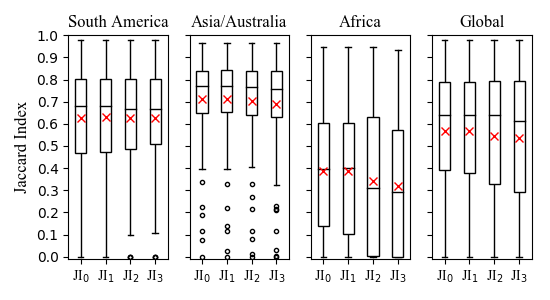
\includegraphics[scale=1]{img/jaccard}
				\caption[Tree cover similarity distribution of the continental regions]{\textbf{Tree cover similarity distribution over the continental regions:} This boxplot shows the distribution of computed Jaccard Index for each raster image tile pair of GlobeLand30 and Global Forest Change tree cover from 2000. The labels $JI_0$, $JI_1$, $JI_2$, and $JI_3$ on the x-axis account for the canopy density classes (0,100], (10,100], (20,100], and (30,100], respectively. The y-axis is the computed Jaccard Index for the corresponding raster image pair, where 0 is a total disagreement and 1 a total agreement. Red crosses within the $Q_{25}$, $Q_{50}$, and $Q_{75}$ boxes highlight the sample mean. Whiskers are 1.5 times the $IQR$.}
				\label{fig:jaccard}
			\end{figure}
			\begin{table}[ht]
				\centering
				\caption[Two-sided Wilcoxon signed-rank test]{\textbf{Two-sided Wilcoxon signed-rank test:}}
				\label{tab:wilcoxontwosided}
				\begin{tabular}{lllllllllllll}
					\hline
					& \multicolumn{12}{c}{H$_0$: $\tilde{x_1}=\tilde{x_2}$} \\\hline
					& \multicolumn{4}{c}{Americas} & \multicolumn{4}{c}{Asia} & \multicolumn{4}{c}{Africa} \\
					Cls & JI$_0$ & JI$_1$ & JI$_2$ & JI$_3$ & JI$_0$ & JI$_1$ & JI$_2$ & JI$_3$ & JI$_0$ & JI$_1$ & JI$_2$ & JI$_3$ \\\hline
					JI$_0$ & - & - & - & - & - & - & - & - & - & - & - & - \\
					JI$_1$ & .00$^{***}$ & - & - & - & .72 & - & - & - & .22 & - & - & - \\
					JI$_2$ & .06 & .36 & - & - & .00$^{***}$ & .00$^{***}$ & - & - & .03$^{*}$ & .03$^{*}$  & - & - \\
					JI$_3$ & .16 & .50 & .60 & - & .00$^{***}$ & .00$^{***}$ & .00$^{***}$ & - & .00$^{***}$ & .00$^{***}$ & .00$^{***}$ & - \\\hline
				\end{tabular}
			\end{table}
			\begin{table}[ht]
				\centering
				\caption[One-sided Wilcoxon signed-rank test]{\textbf{One-sided Wilcoxon signed-rank test:}}
				\label{tab:wilcoxononesided}
				\begin{tabular}{llllllllllllll}
					\hline
					& & \multicolumn{12}{c}{H$_0$: $\tilde{x_1}\leq\tilde{x_2}$} \\\hline
					& & \multicolumn{4}{c}{Americas} & \multicolumn{4}{c}{Asia} & \multicolumn{4}{c}{Africa} \\
					& Cls & JI$_0$ & JI$_1$ & JI$_2$ & JI$_3$ & JI$_0$ & JI$_1$ & JI$_2$ & JI$_3$ & JI$_0$ & JI$_1$ & JI$_2$ & JI$_3$ \\\hline
					\multirow{4}{*}{\STAB{\rotatebox[origin=c]{90}{H$_0$: $\tilde{x_1}\geq\tilde{x_2}$}}} & JI$_0$ & - & .00$^{****}$ & .03$^{*}$ & .08 & - & .64 & 1. & 1. & - & .11 & .98 & 1. \\
					& JI$_1$ & 1. & - & .18 & .25 & .36 & - & 1. & 1. & .89 & - & .99 & 1. \\
					& JI$_2$ & .97 & .82 & - & .30 & .00$^{****}$ & .00$^{****}$ & - & 1. & .02 & .01 & - & 1. \\
					& JI$_3$ & .92 & .75 & .70 & - & .00$^{****}$ & .00$^{****}$ & .00$^{****}$ & - & .00 & .00 & .00 & - \\\hline
				\end{tabular}
			\end{table}

		\subsection{Tree cover and deforestation}
		\label{subsec:results_tree_cover_and_deforestation}
			\note{Goal:}\note{}

		\subsection{Proximate deforestation driver}
		\label{subsec:results_proxy_deforestation_driver}

		\subsection{Accuracy assessment}
		\label{subsec:results_accuracy_assessment}
			\begin{table}[ht]
				\centering
				\caption[Accuracy assessment]{Confusion matrix for accuracy assessment}
				\label{tab:accuracy}
				\begin{tabular}{llrrrrrrrrrrrr}
					\hline
					& & \multicolumn{9}{c}{Reference} & & & \\
					& Cls & 10 & 20 & 25 & 30 & 40 & 50 & 60 & 80 & 90 & Tot & UAc & Om \\\hline
					\multirow{9}{*}{\STAB{\rotatebox[origin=c]{90}{Prediction}}}
					& 10 & 732 & 38 & 62 & 15 & 16 & 2 & 3 & 5 & 0 & 873 & .84 & .16 \\ 
					& 20 & 42 & 751 & 57 & 189 & 31 & 12 & 0 & 17 & 4 & 1103 & .68 & .32 \\ 
					& 25 & 29 & 202 & 1155 & 173 & 22 & 10 & 5 & 11 & 4 & 1611 & .72 & .28 \\ 
					& 30 & 36 & 187 & 32 & 1466 & 73 & 21 & 0 & 17 & 0 & 1832 & .80 & .20 \\ 
					& 40 & 14 & 21 & 4 & 41 & 352 & 1 & 1 & 2 & 1 & 437 & .81 & .19 \\ 
					& 50 & 0 & 5 & 3 & 10 & 4 & 50 & 0 & 1 & 0 & 73 & .68 & .32 \\ 
					& 60 & 2 & 1 & 0 & 3 & 0 & 2 & 18 & 2 & 0 & 28 & .64 & .36 \\ 
					& 80 & 3 & 4 & 0 & 1 & 1 & 1 & 0 & 50 & 0 & 60 & .83 & .17 \\ 
					& 90 & 0 & 0 & 0 & 1 & 0 & 0 & 0 & 3 & 5 & 9 & .56 & .44 \\\hline 
					& Tot & 858 & 1209 & 1313 & 1899 & 499 & 99 & 27 & 108 & 14 & 6026 & & \\
					& PAc & .85 & .62 & .88 & .77 & .71 & .51 & .67 & .46 & .36 & & \multicolumn{2}{r}{OvAc} \\
					& Com & .15 & .38 & .12 & .23 & .29 & .49 & .33 & .54 & .64 & & \multicolumn{2}{r}{.75} \\ \hline
				\end{tabular}
			\end{table}

	\section{Emissions}

	\section{Ecosystem service values}




%%%%%%% TABLE AND FIGURES

%			\begin{table}[ht]
%				\centering
%				\caption[Deforestation driver]{Absolute in km$^2$}
%				\label{tab:driver_tab}
%				\begin{tabular}{lcllrrr}
%					Class & Code & Type & & Americas & Asia & Africa \\\hline
%					\multirow{4}{*}{Agriculture} & \multirow{2}{*}{10} & \multirow{2}{*}{Cropland} & rel. & 24.37 & 18.37 & 25.01 \\
%					& & & abs. & 95908 & 38719 & 44368 \\
%					& \multirow{2}{*}{30} & \multirow{2}{*}{Grassland} & rel. & 46.19 & 8.41 & 50.46 \\
%					& & & abs. & 181781 & 17726 & 89516 \\
%					\multirow{4}{*}{Forestry/Plantations} & \multirow{2}{*}{25} & \multirow{2}{*}{Regrowth} & rel. & 14.40 & 70.27 & 18.61 \\
%					& & & abs. & 56671 & 148111 & 33014 \\
%					& \multirow{2}{*}{40} & \multirow{2}{*}{Shrubland} & rel. & 12.69 & 1.11 & 3.77 \\
%					& & & abs. & 49941 & 2340 & 6688 \\
%					\multirow{4}{*}{Urban/Mining} & \multirow{2}{*}{80} & \multirow{2}{*}{Artificial} & rel. & 0.41 & 0.46 & 0.71 \\
%					& & & abs. & 1614 & 970 & 1260 \\
%					& \multirow{2}{*}{90} & \multirow{2}{*}{Bareland} & rel. & 0.10 & 0.03 & 0.09 \\
%					& & & abs. & 394 & 63 & 160 \\
%					\multirow{4}{*}{Natural} & \multirow{2}{*}{50} & \multirow{2}{*}{Wetland} & rel. & 1.50 & 0.97 & 1.23 \\
%					& & & abs. & 5903 & 2045 & 2182 \\
%					& \multirow{2}{*}{60} & \multirow{2}{*}{Water} & rel. & 0.32 & 0.38 & 0.13 \\
%					& & & abs. & 1259 & 801 & 231 \\\hline
%					\multicolumn{3}{c}{\multirow{2}{*}{Forest loss}} & rel. & 3.87 & 4.68 & 1.69 \\
%					& & & abs. & 393550 & 210774 & 177400 \\
%					\multicolumn{3}{c}{Forest cover} & abs. & 10223187 & 4457940 & 10496591 \\\hline
%				\end{tabular}
%			\end{table}

% LATIN AMERICA
%			\begin{figure}[ht]
%				\centering
%				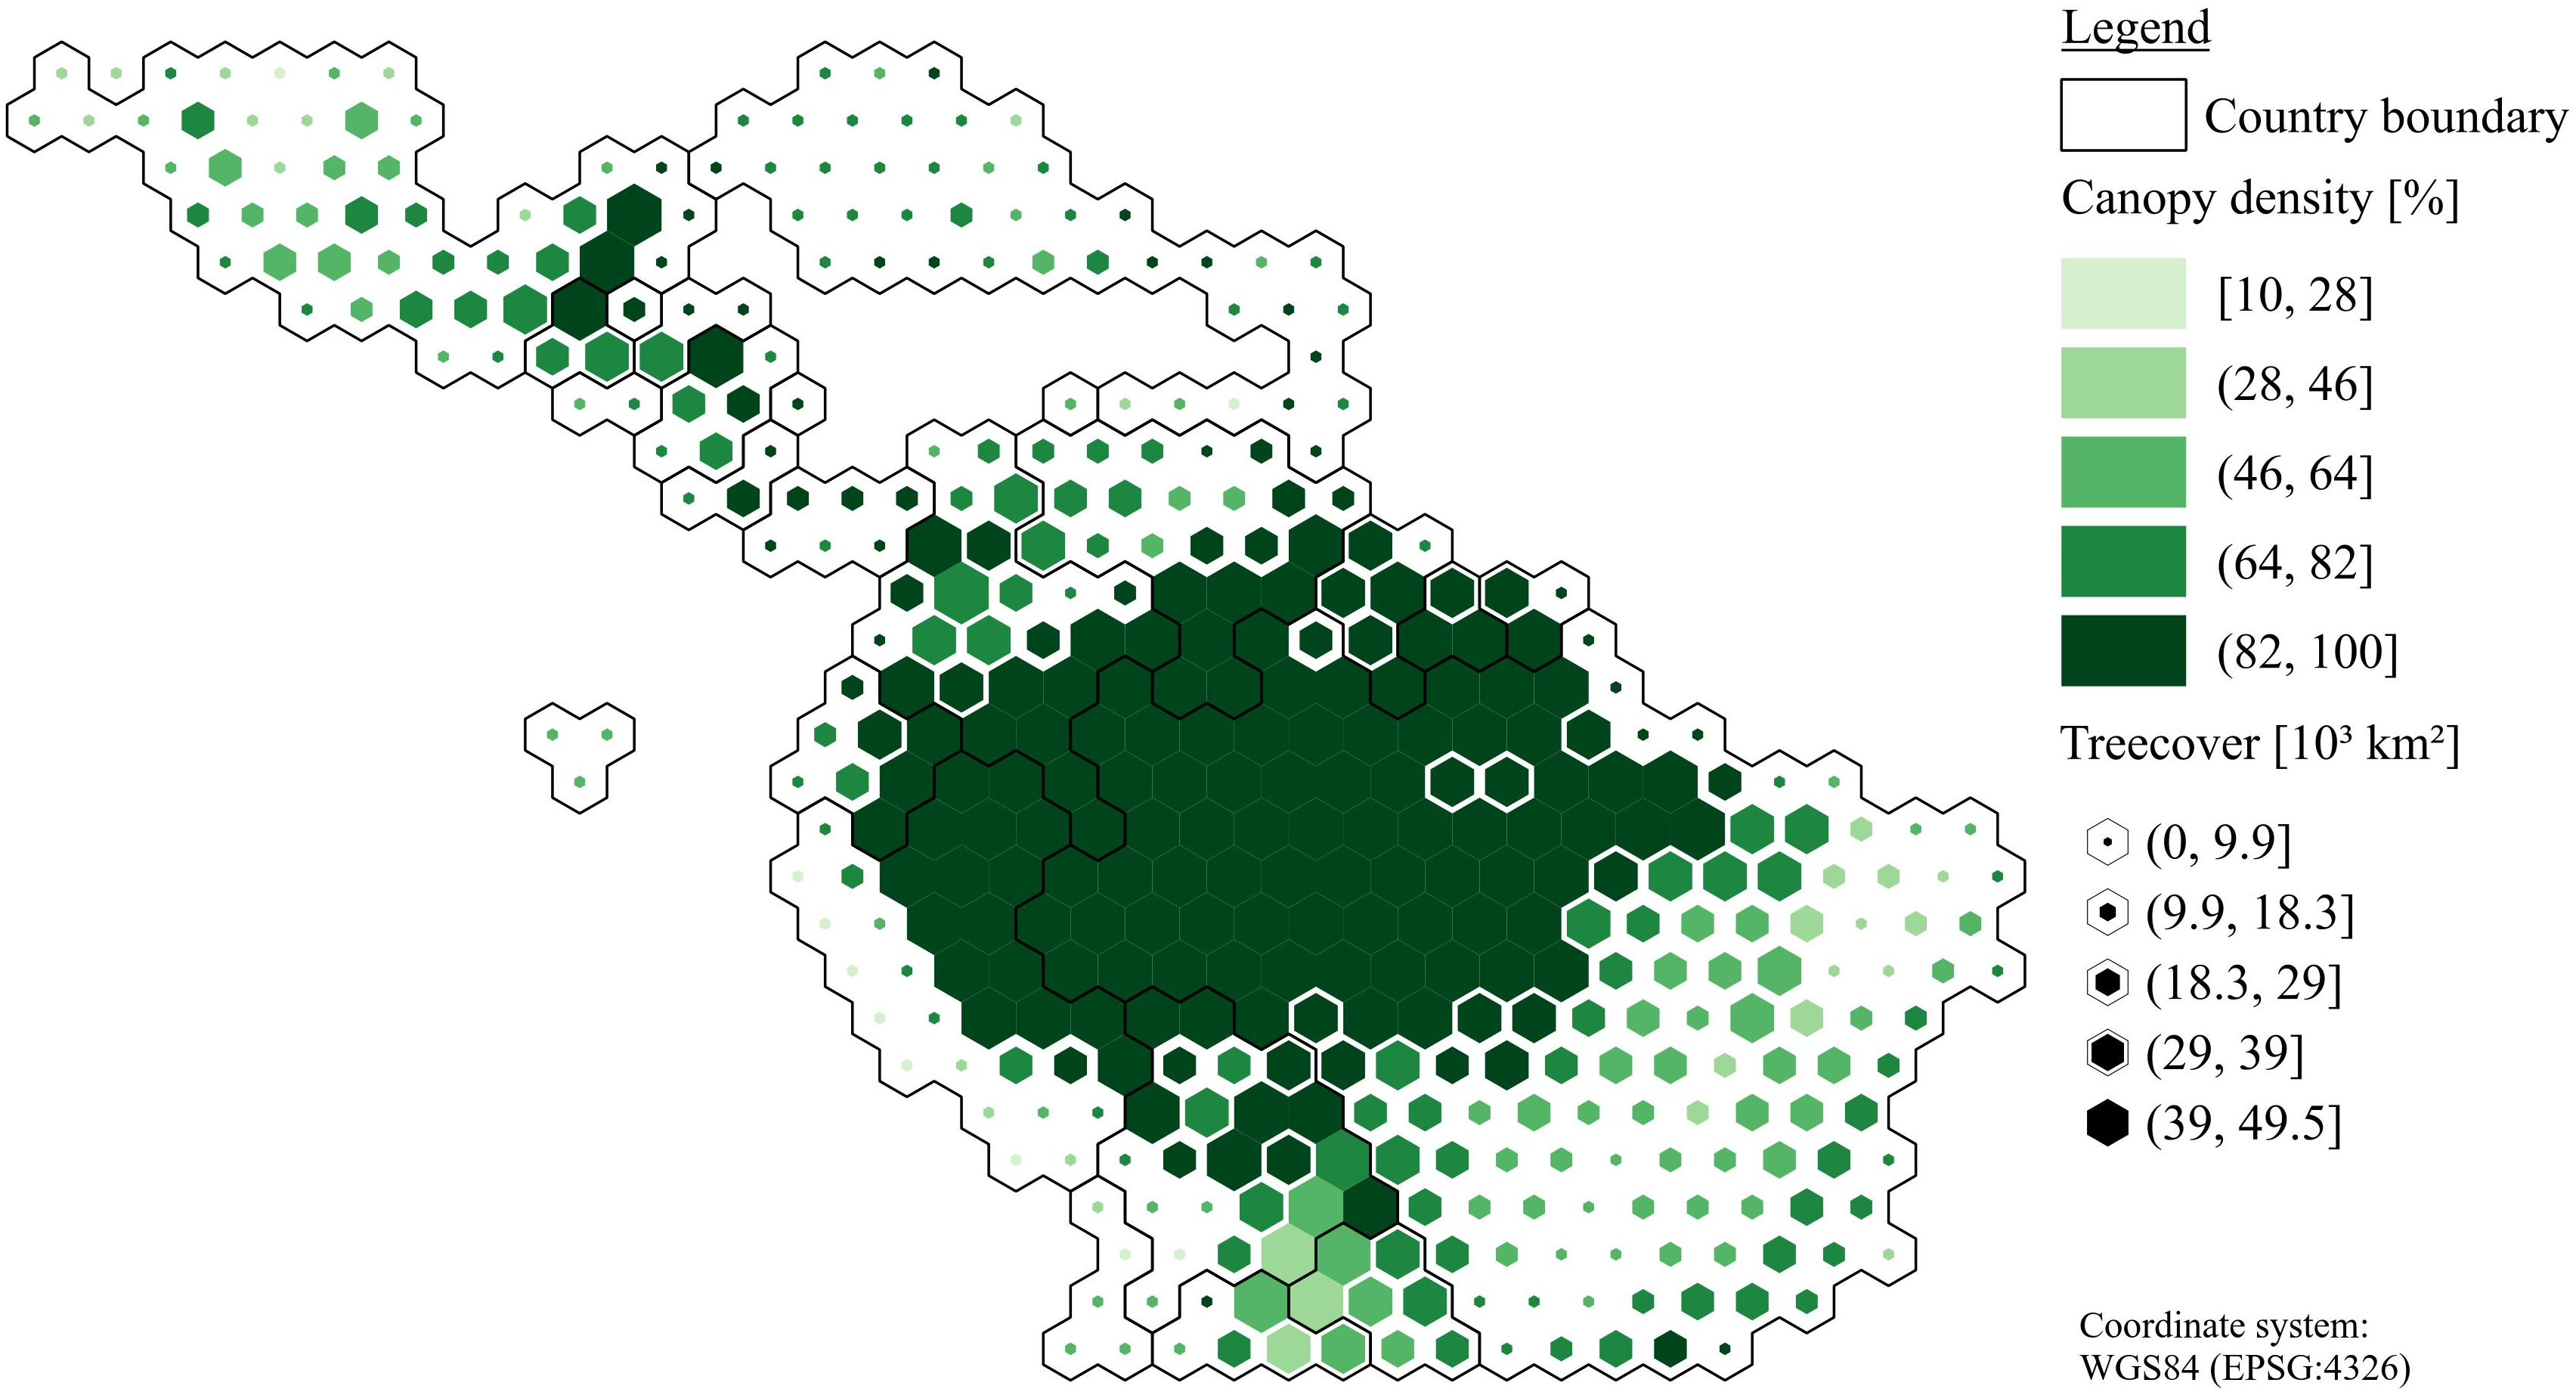
\includegraphics[scale=1]{img/americas_treecover_frameless}
%				\caption[Ecosystem service values]{}
%				\label{fig:americascover}
%			\end{figure}
%			\begin{figure}[ht]
%				\centering
%				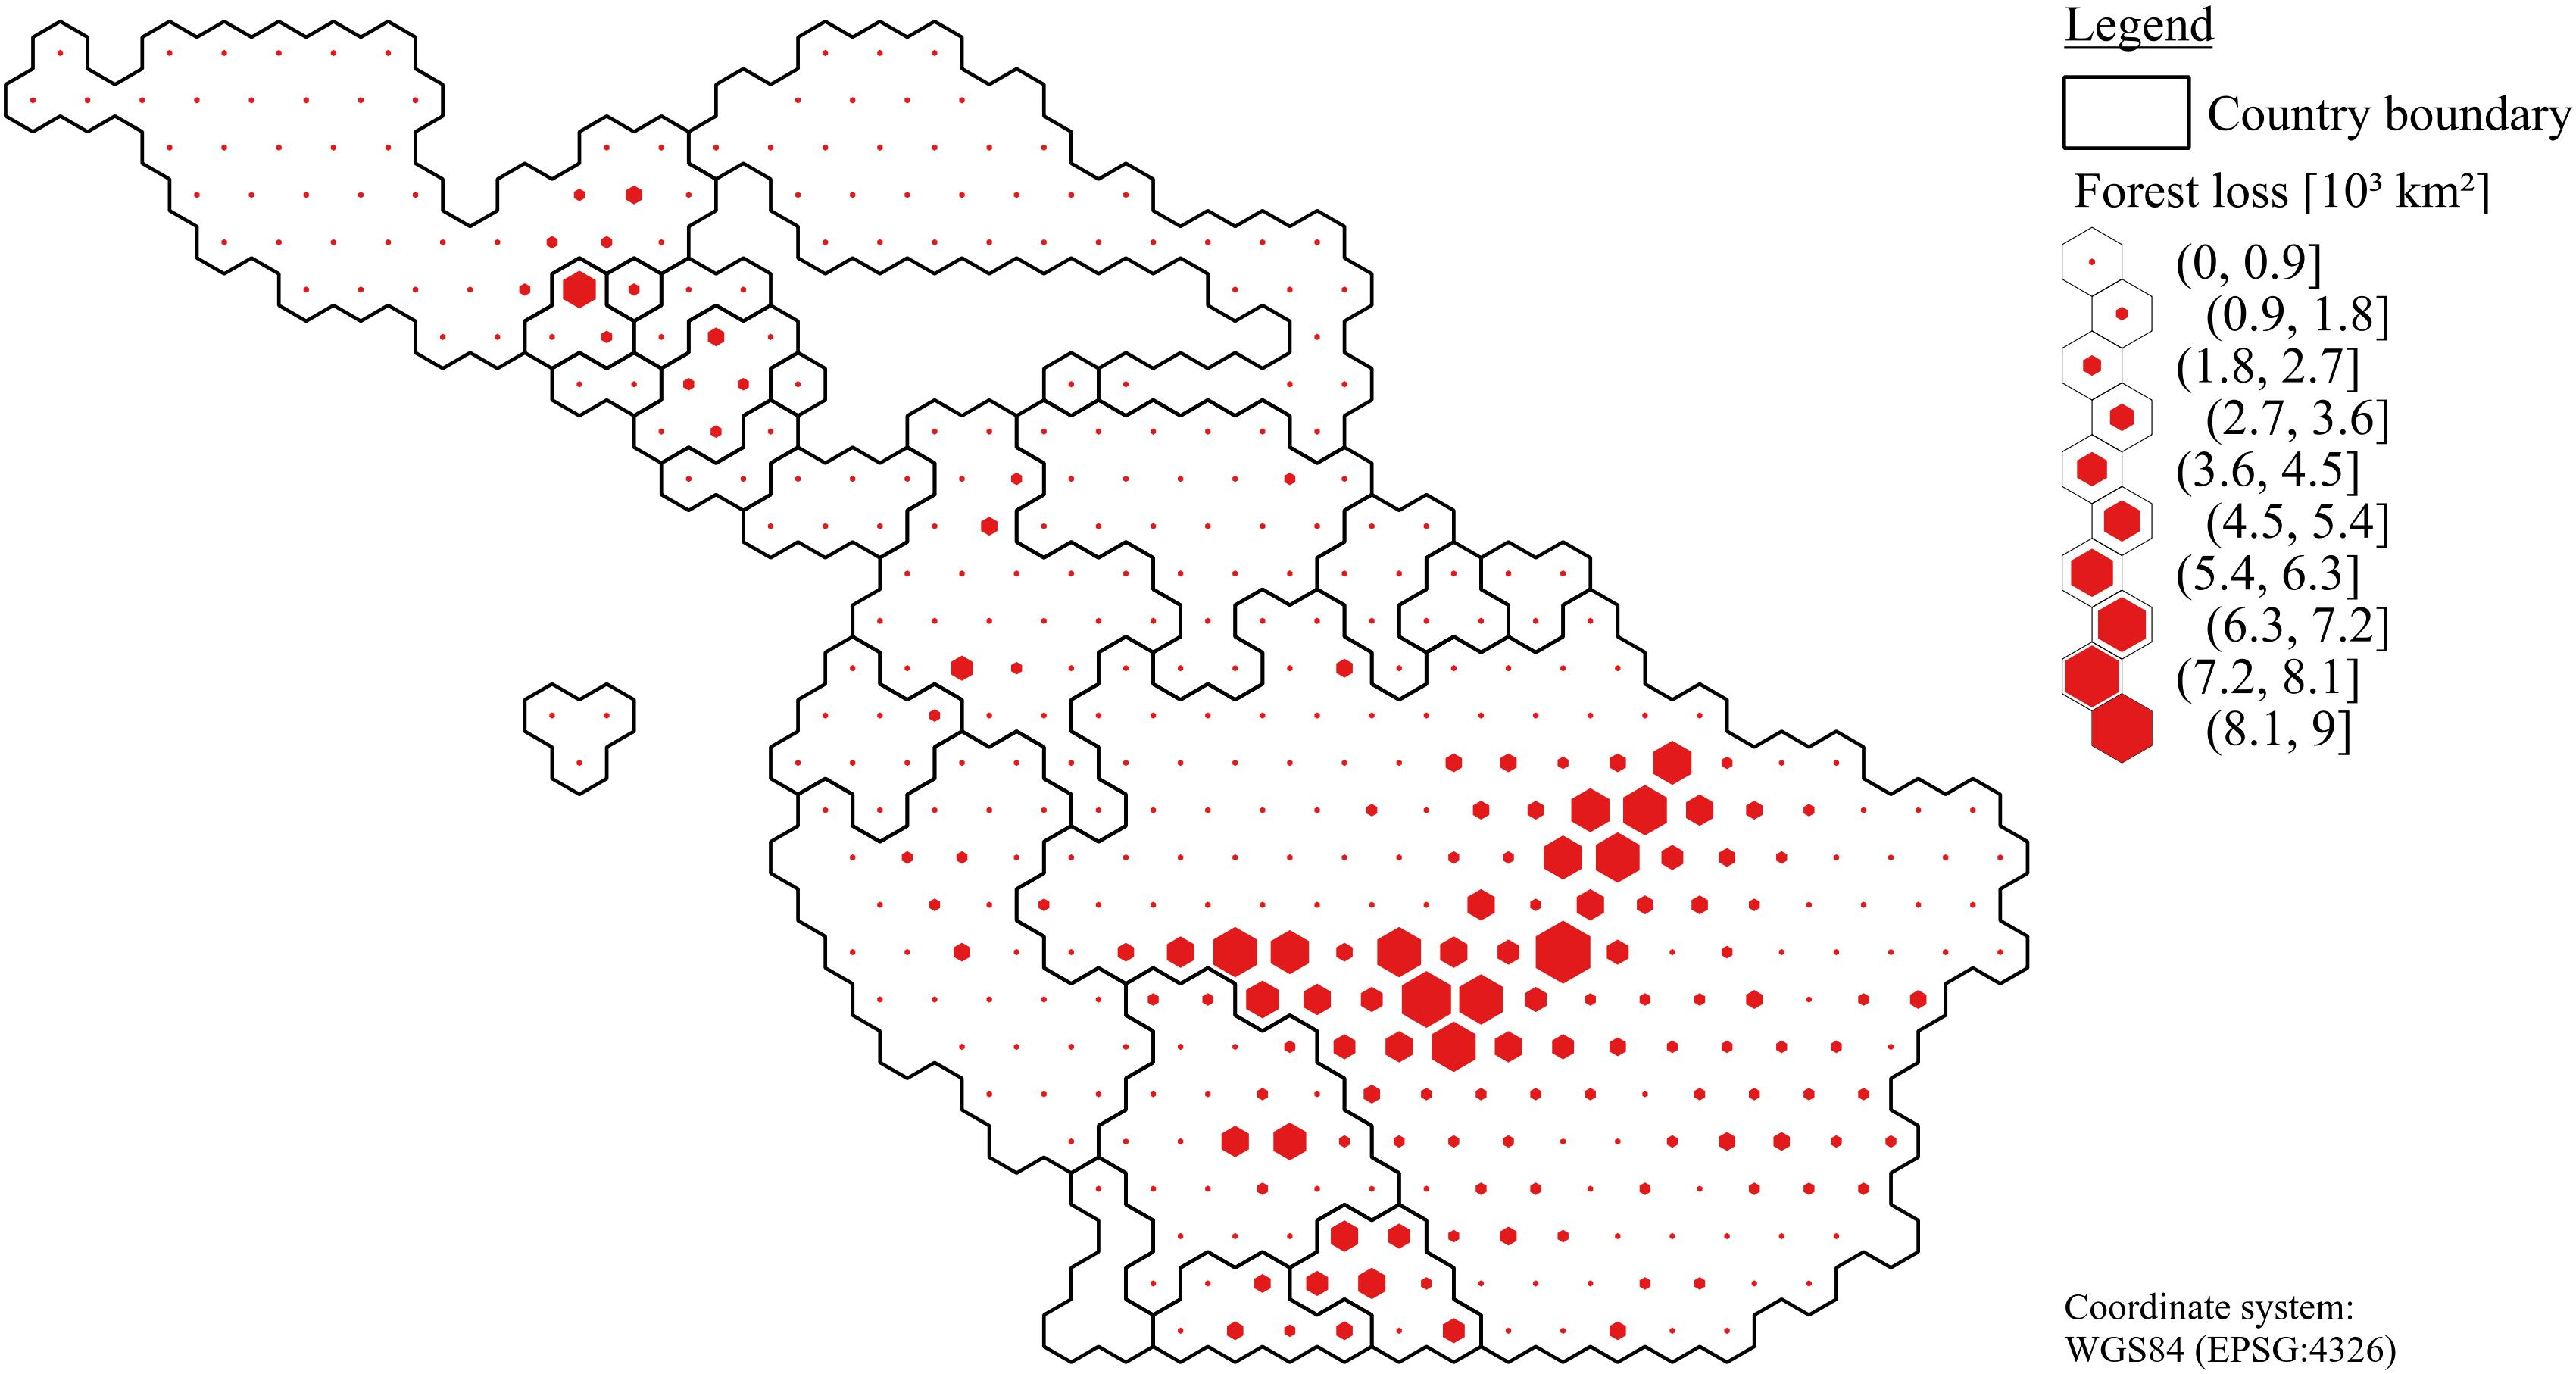
\includegraphics[scale=1]{img/americas_loss_frameless}
%				\caption[Ecosystem service values]{}
%				\label{fig:americasloss}
%			\end{figure}
%			\begin{figure}[ht]
%				\centering
%				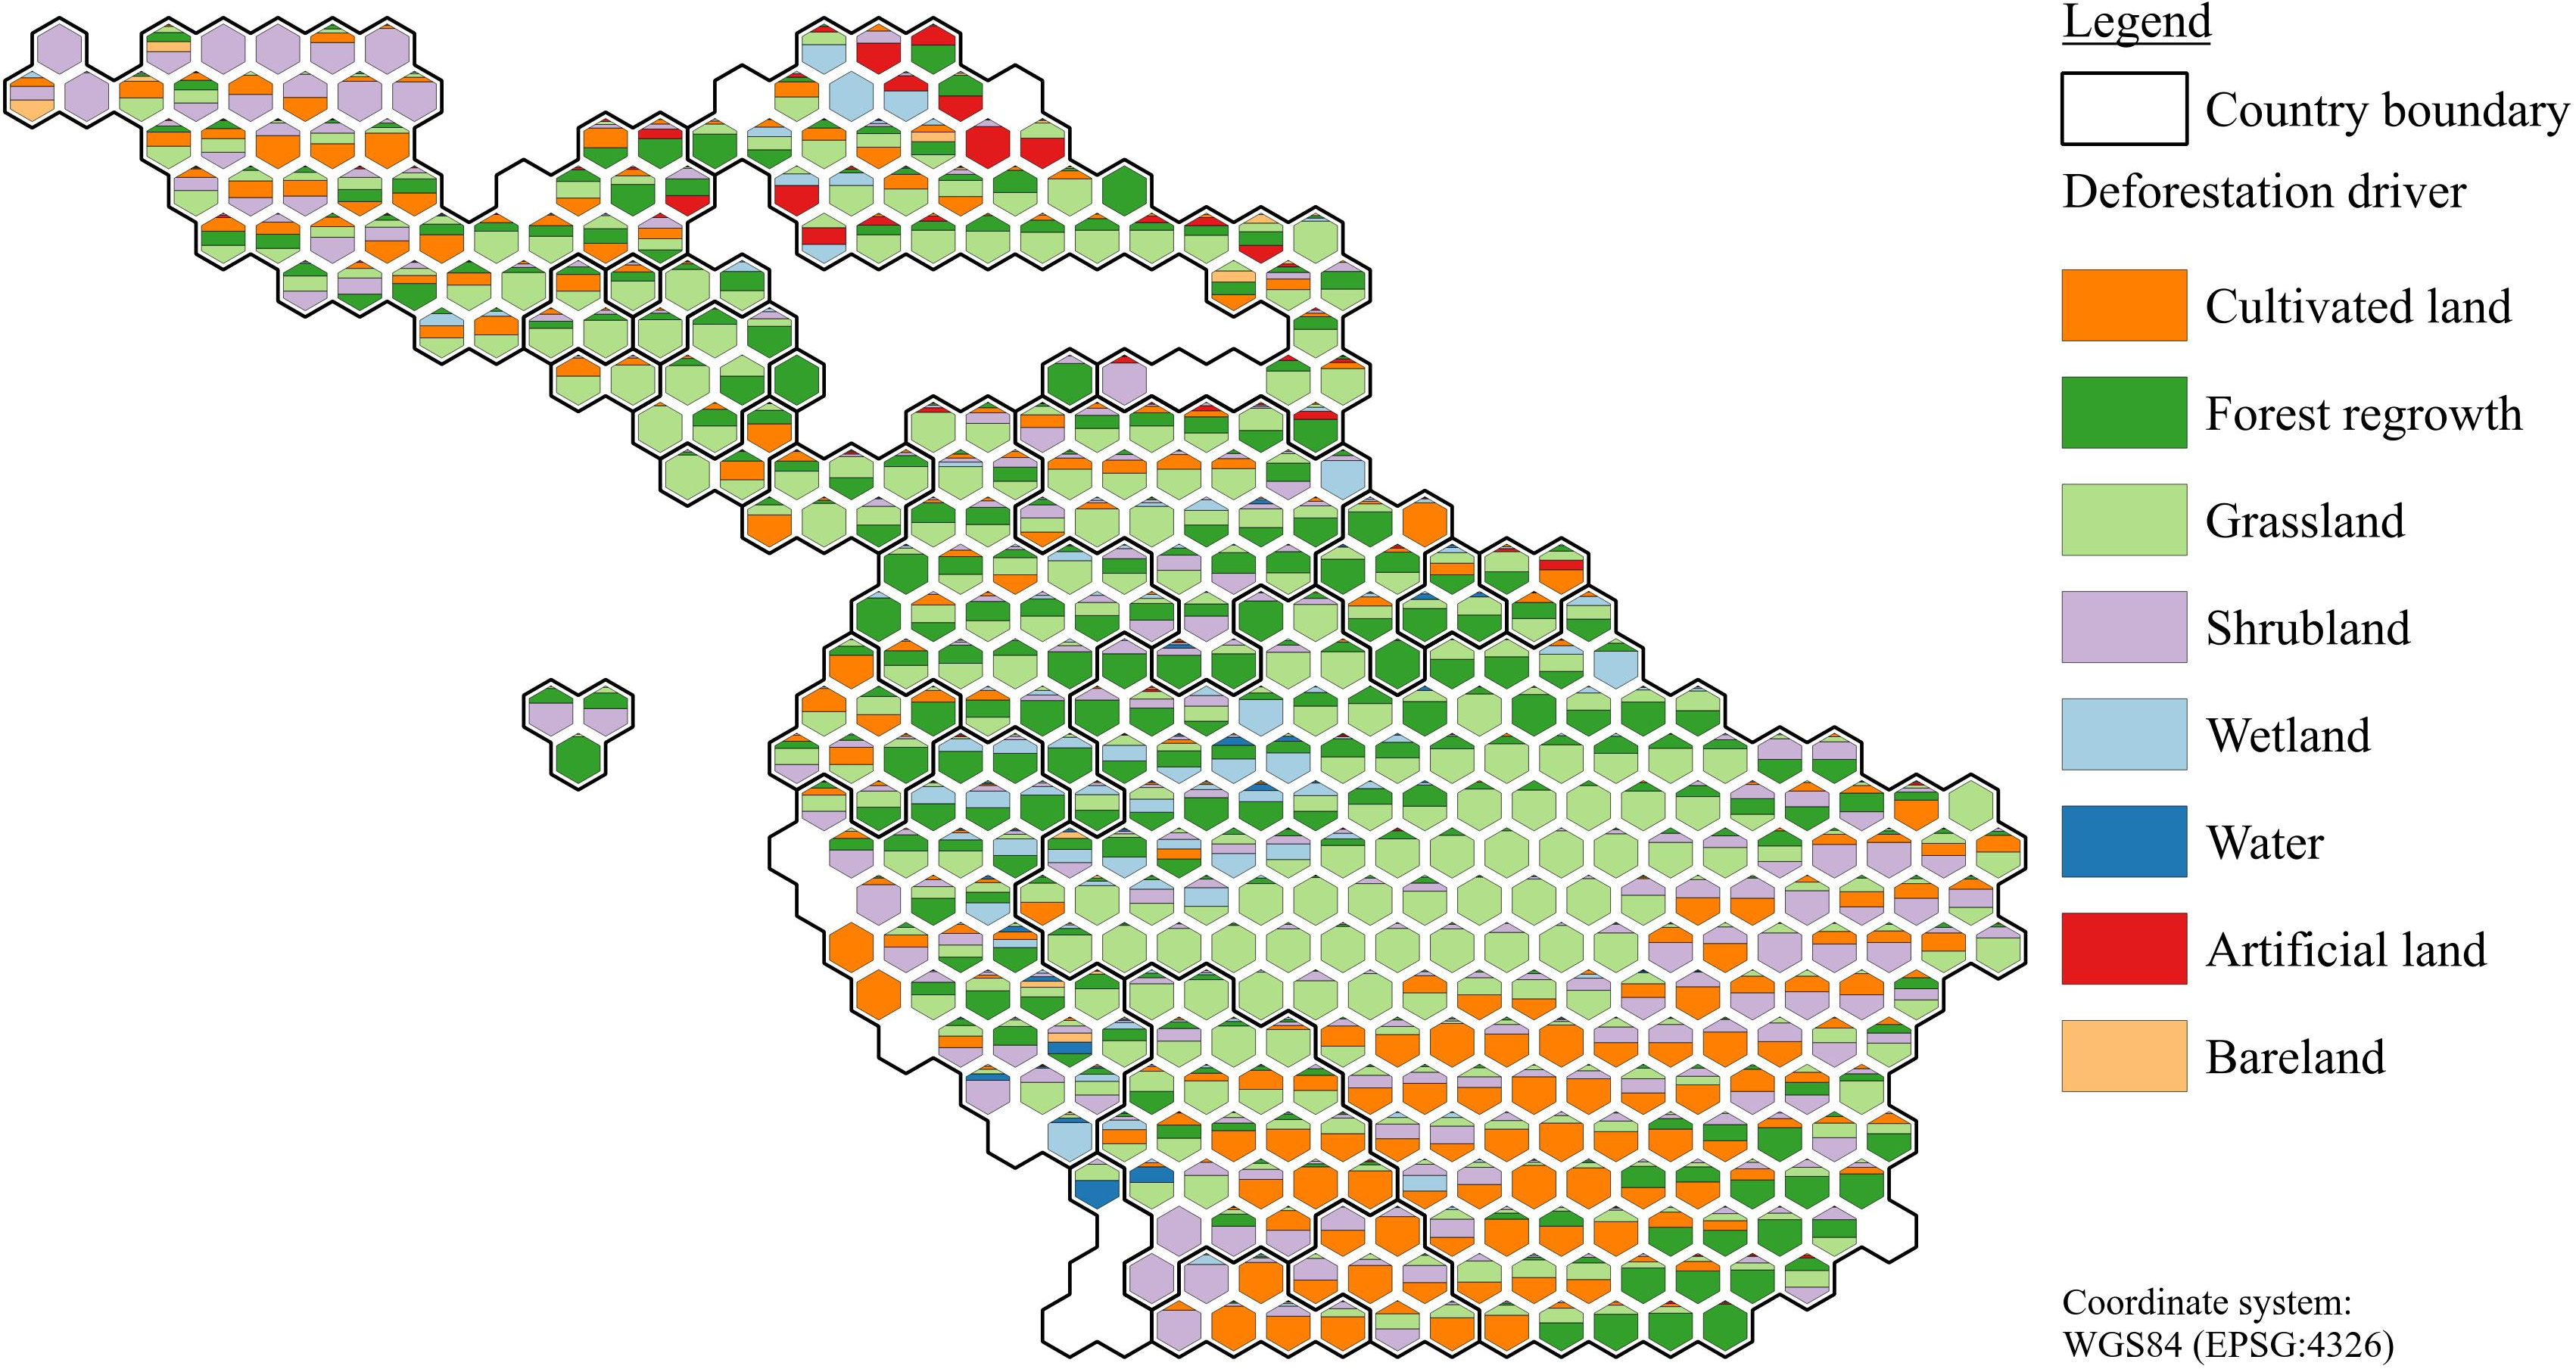
\includegraphics[scale=1]{img/americas_driver_frameless}
%				\caption[Ecosystem service values]{}
%				\label{fig:americasdriver}
%			\end{figure}

% ASIA
%			\begin{figure}[ht]
%				\centering
%				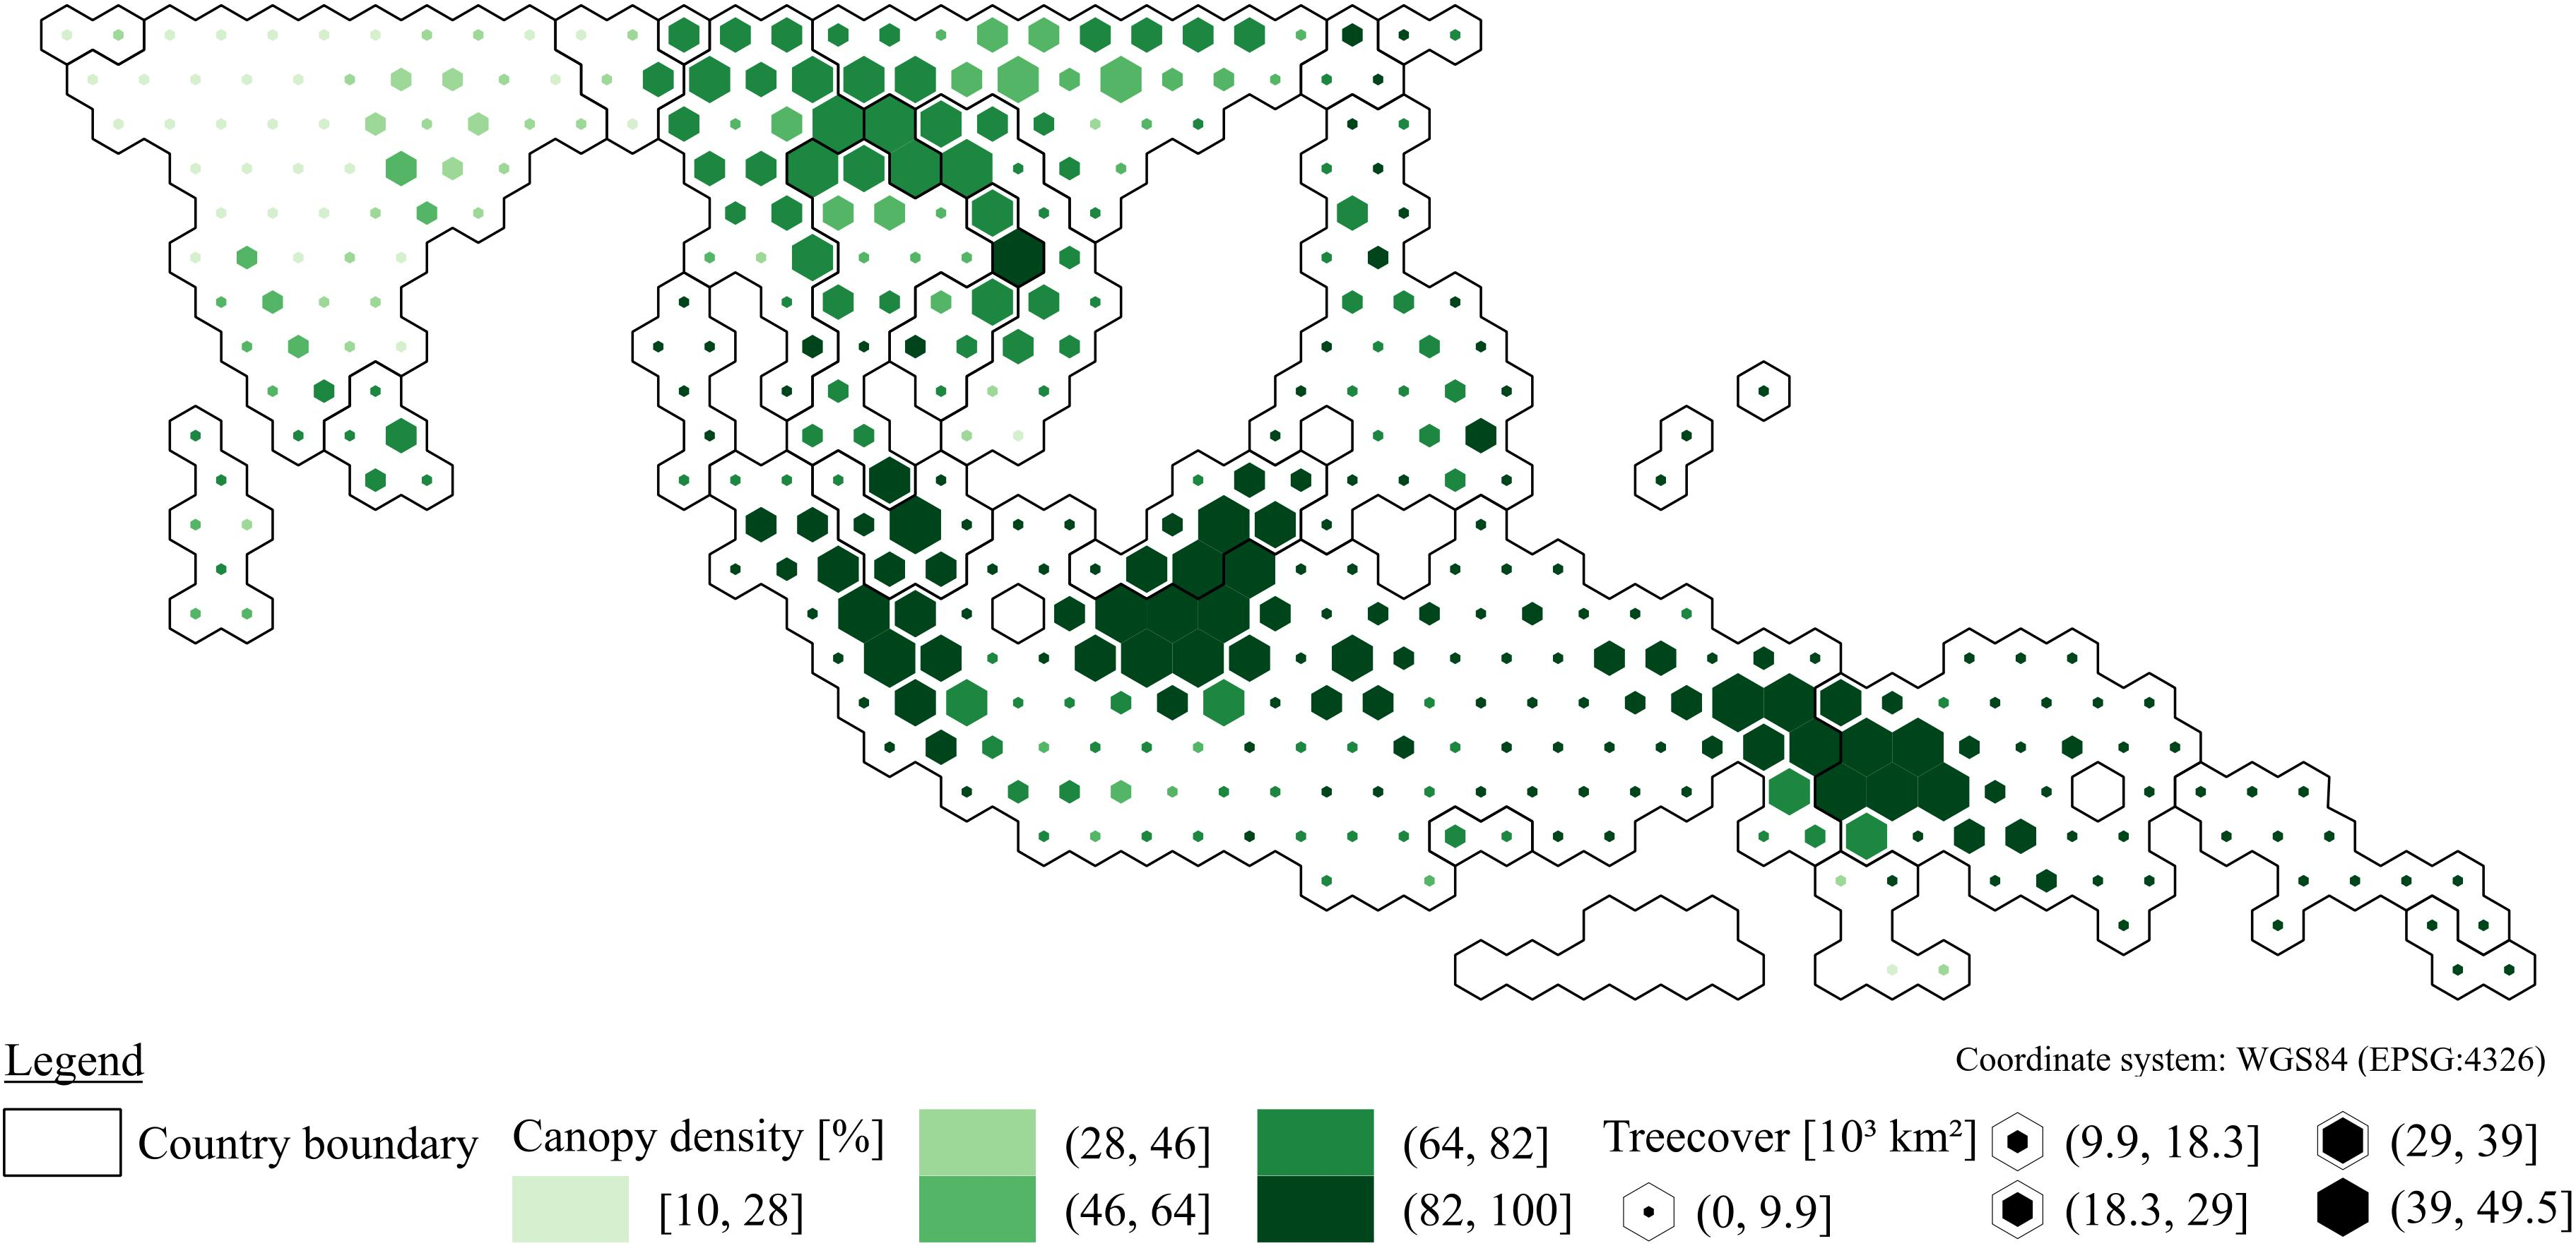
\includegraphics[scale=1]{img/asia_treecover_frameless}
%				\caption[Ecosystem service values]{}
%				\label{fig:asiacover}
%			\end{figure}
%			\begin{figure}[ht]
%				\centering
%				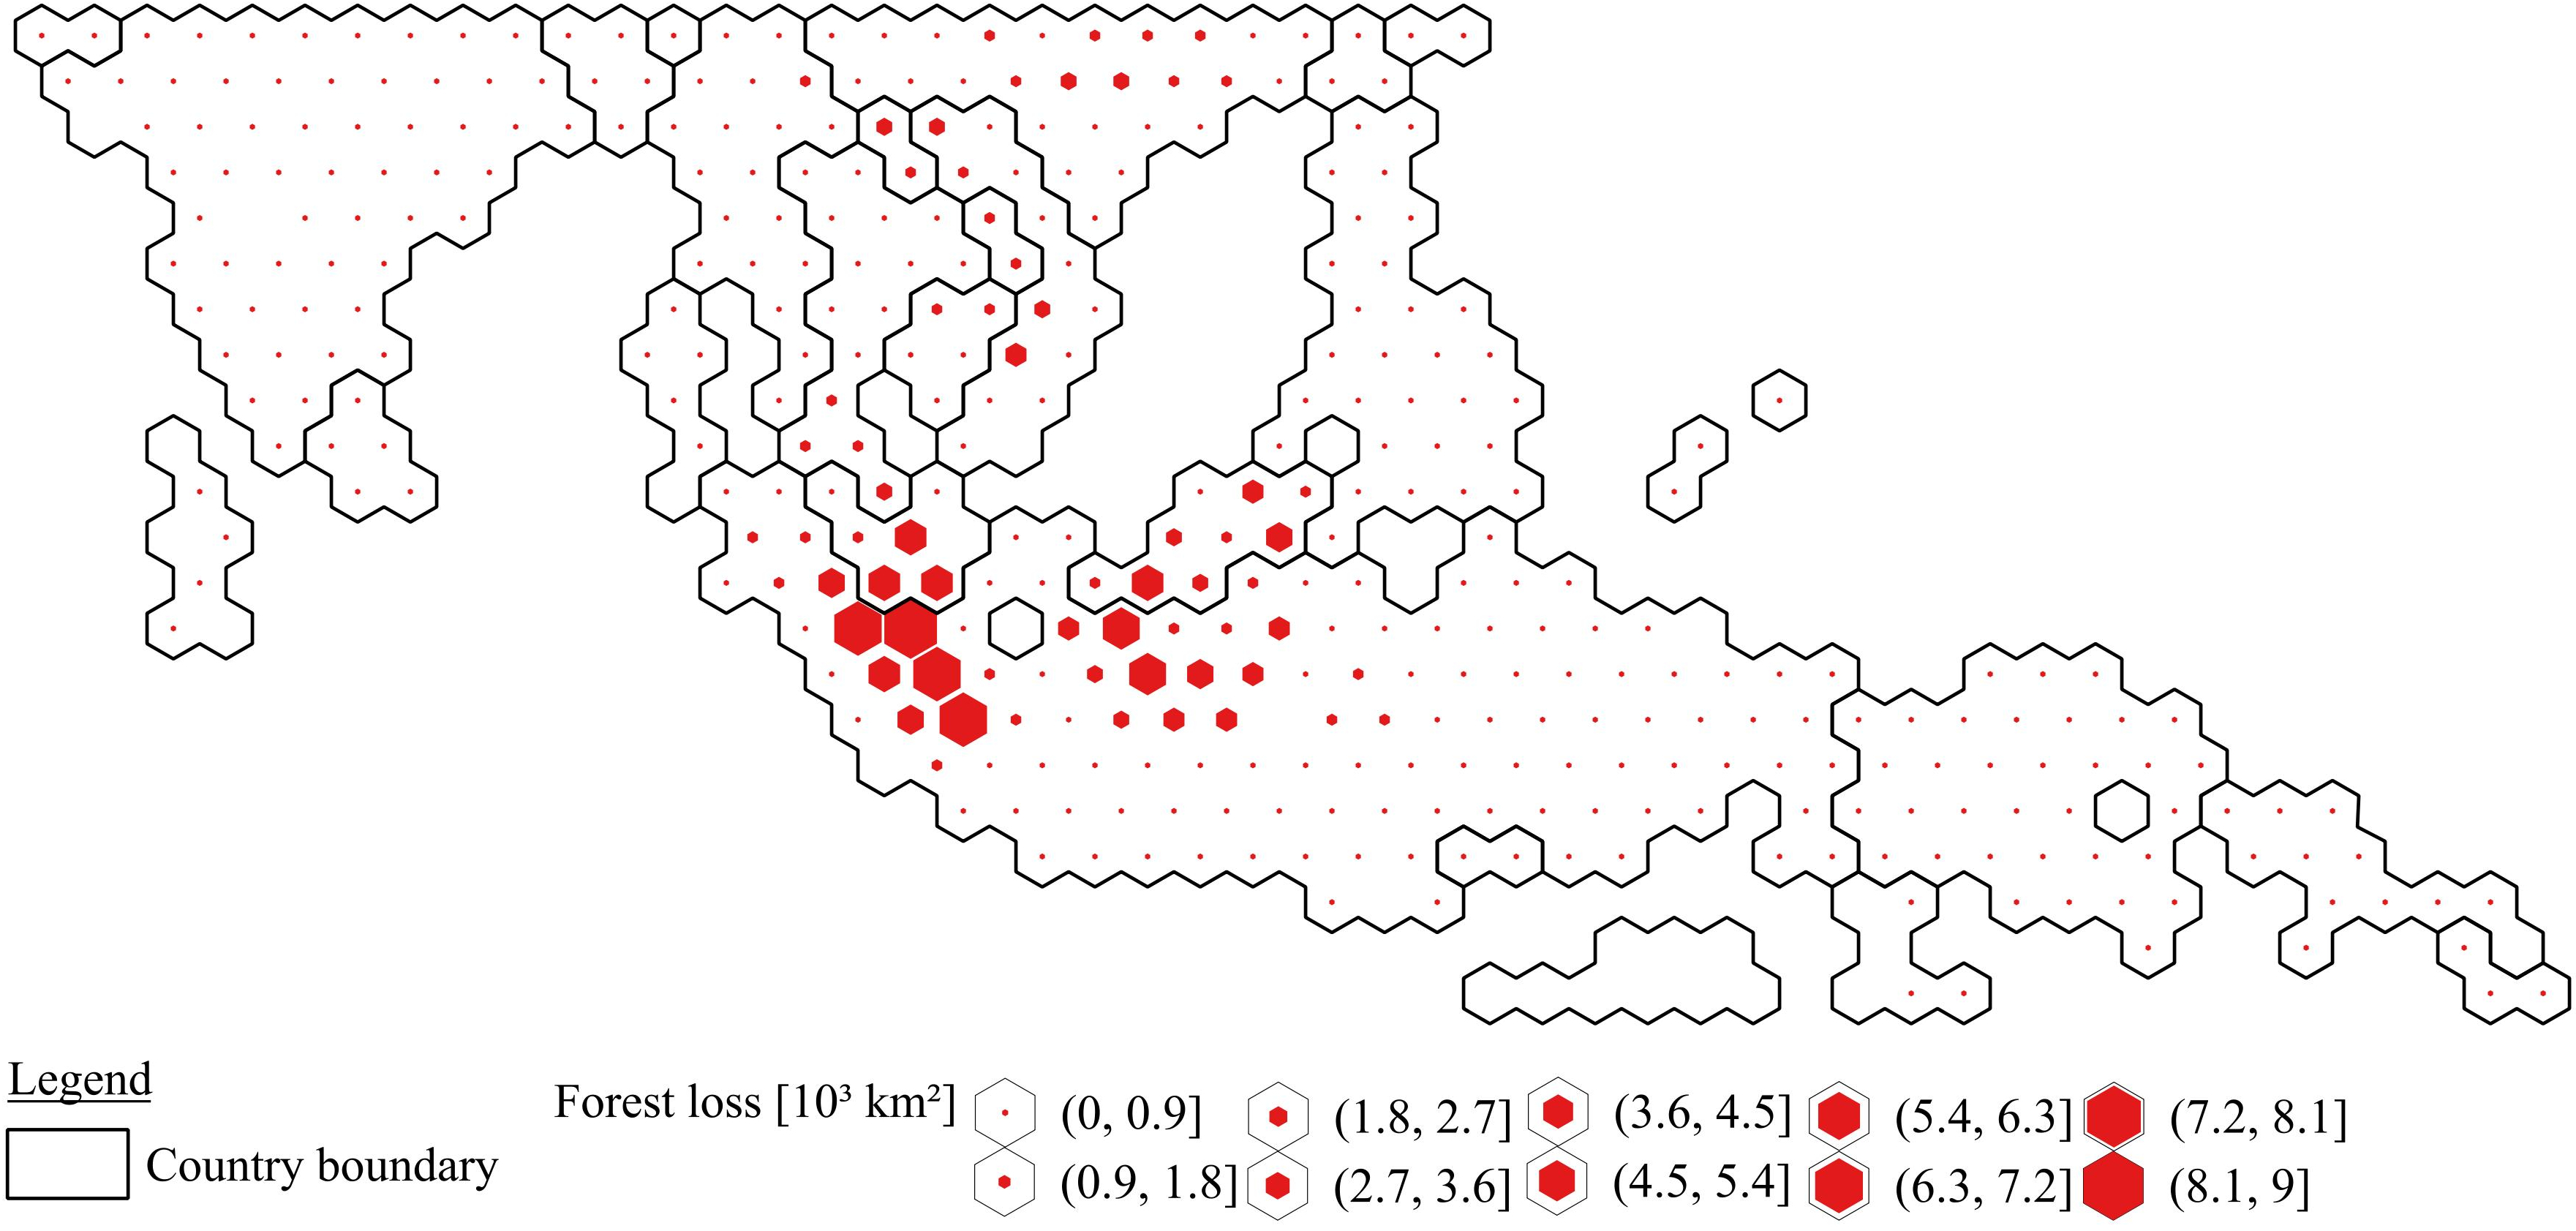
\includegraphics[scale=1]{img/asia_loss_frameless}
%				\caption[Ecosystem service values]{}
%				\label{fig:asialoss}
%			\end{figure}
%			\begin{figure}[ht]
%				\centering
%				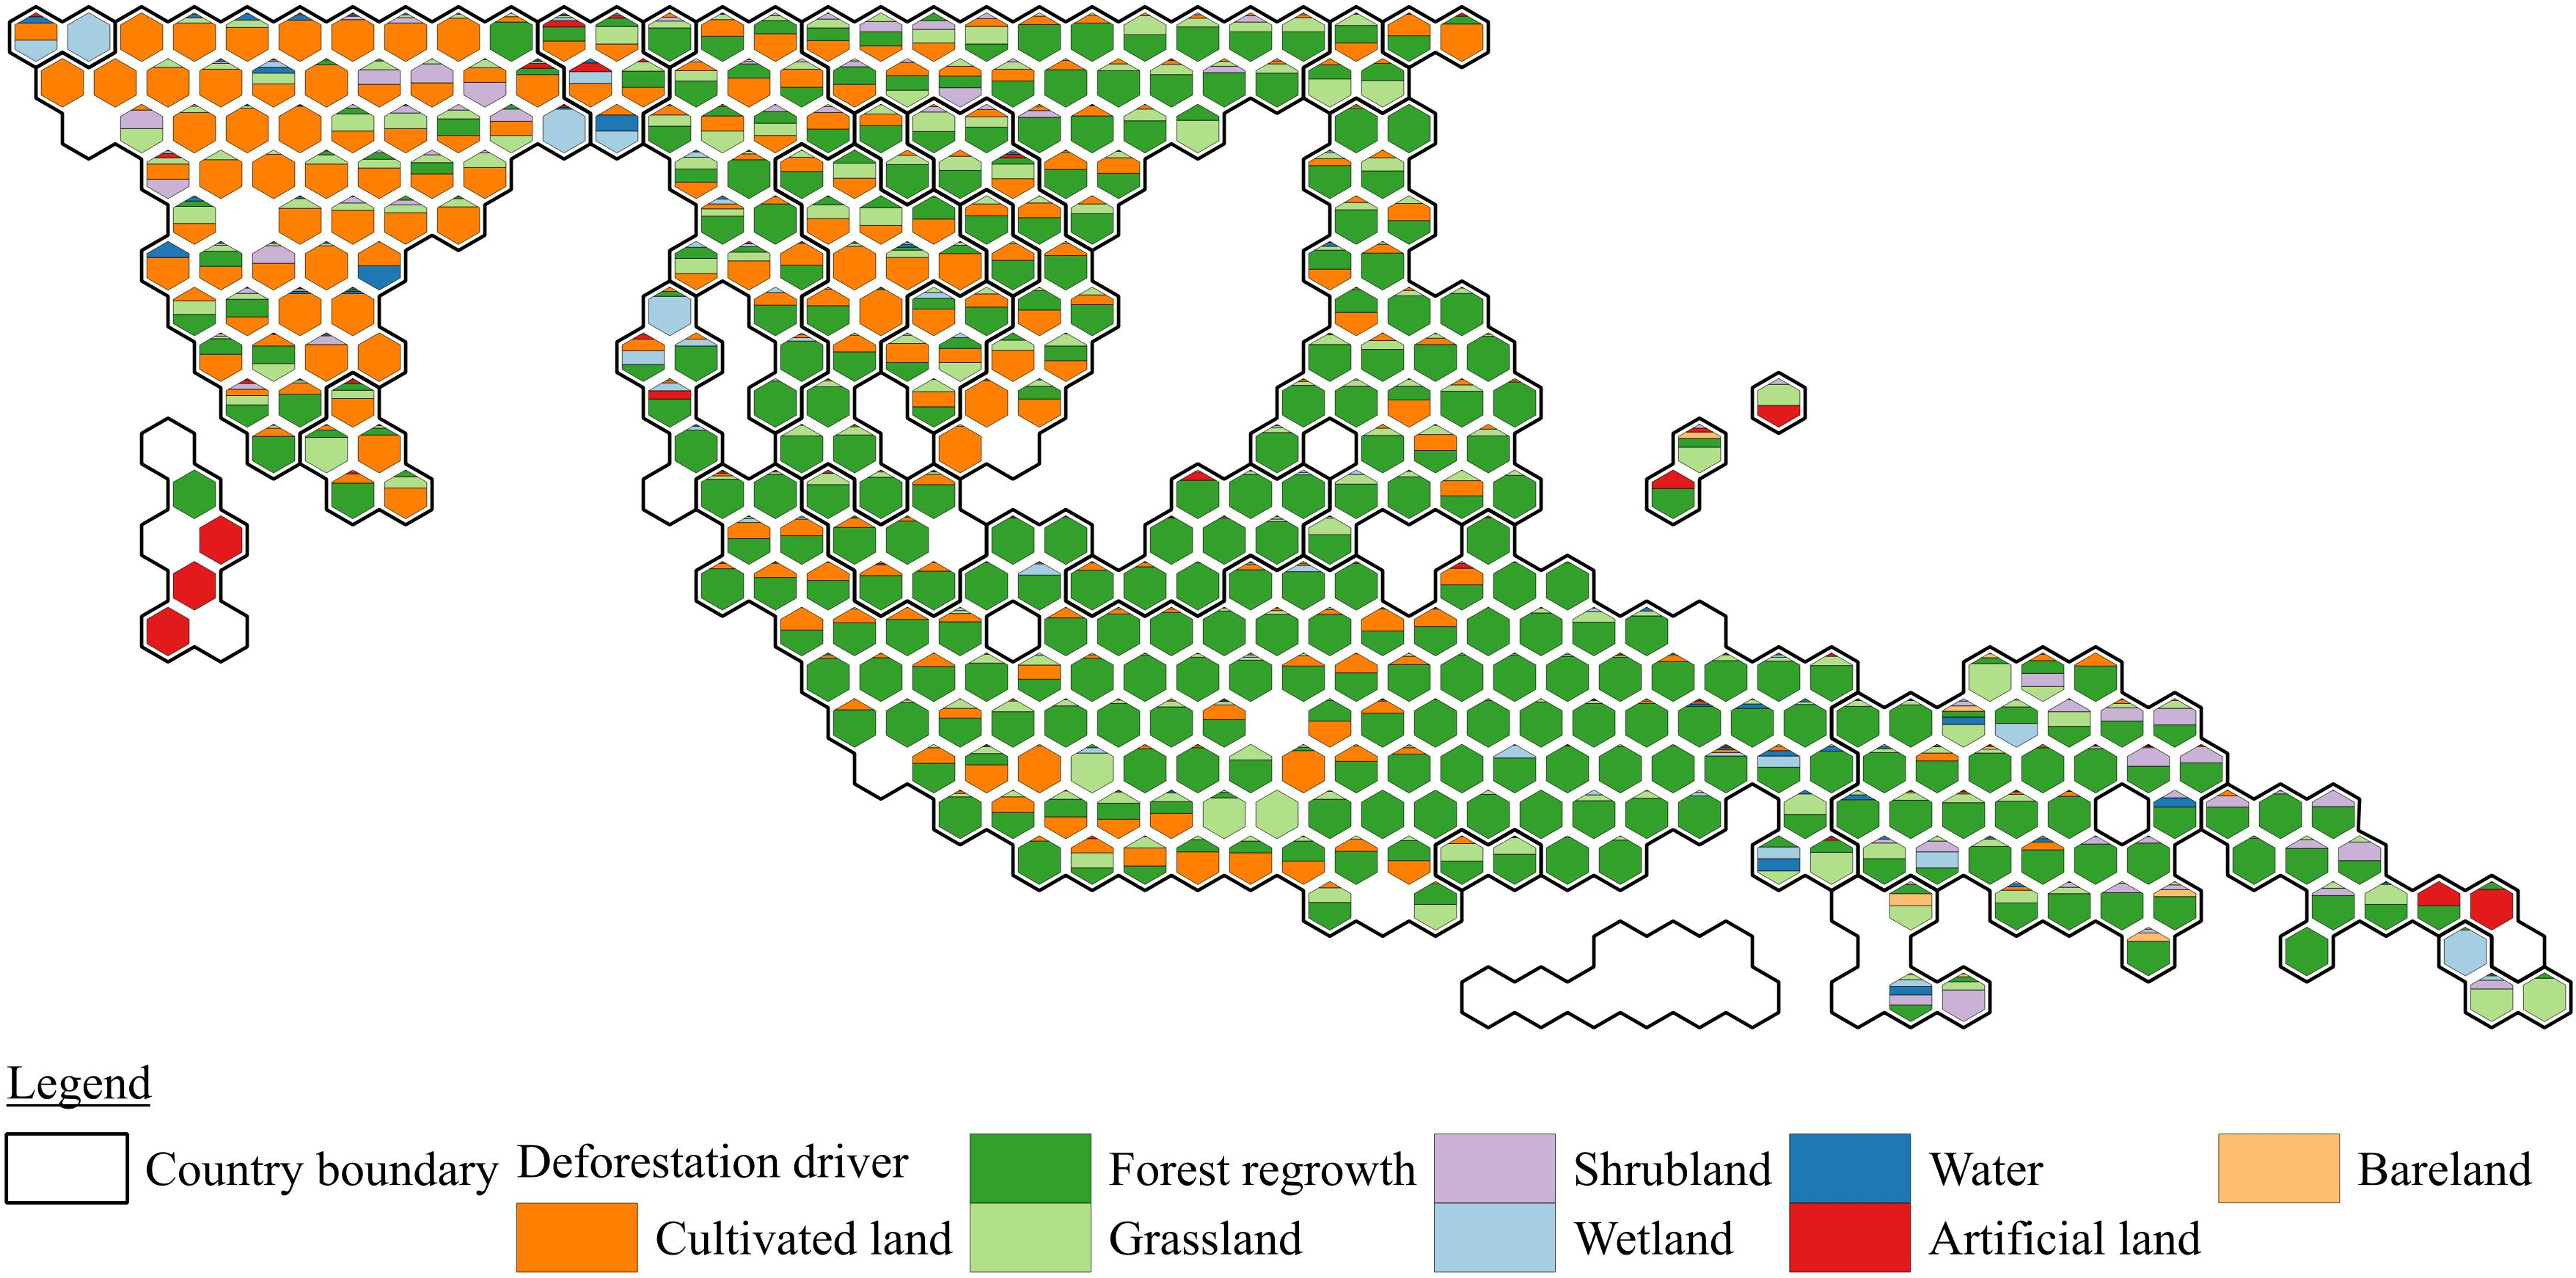
\includegraphics[scale=1]{img/asia_driver_frameless}
%				\caption[Ecosystem service values]{}
%				\label{fig:asiadriver}
%			\end{figure}

% AFRICA
%			\begin{figure}[ht]
%				\centering
%				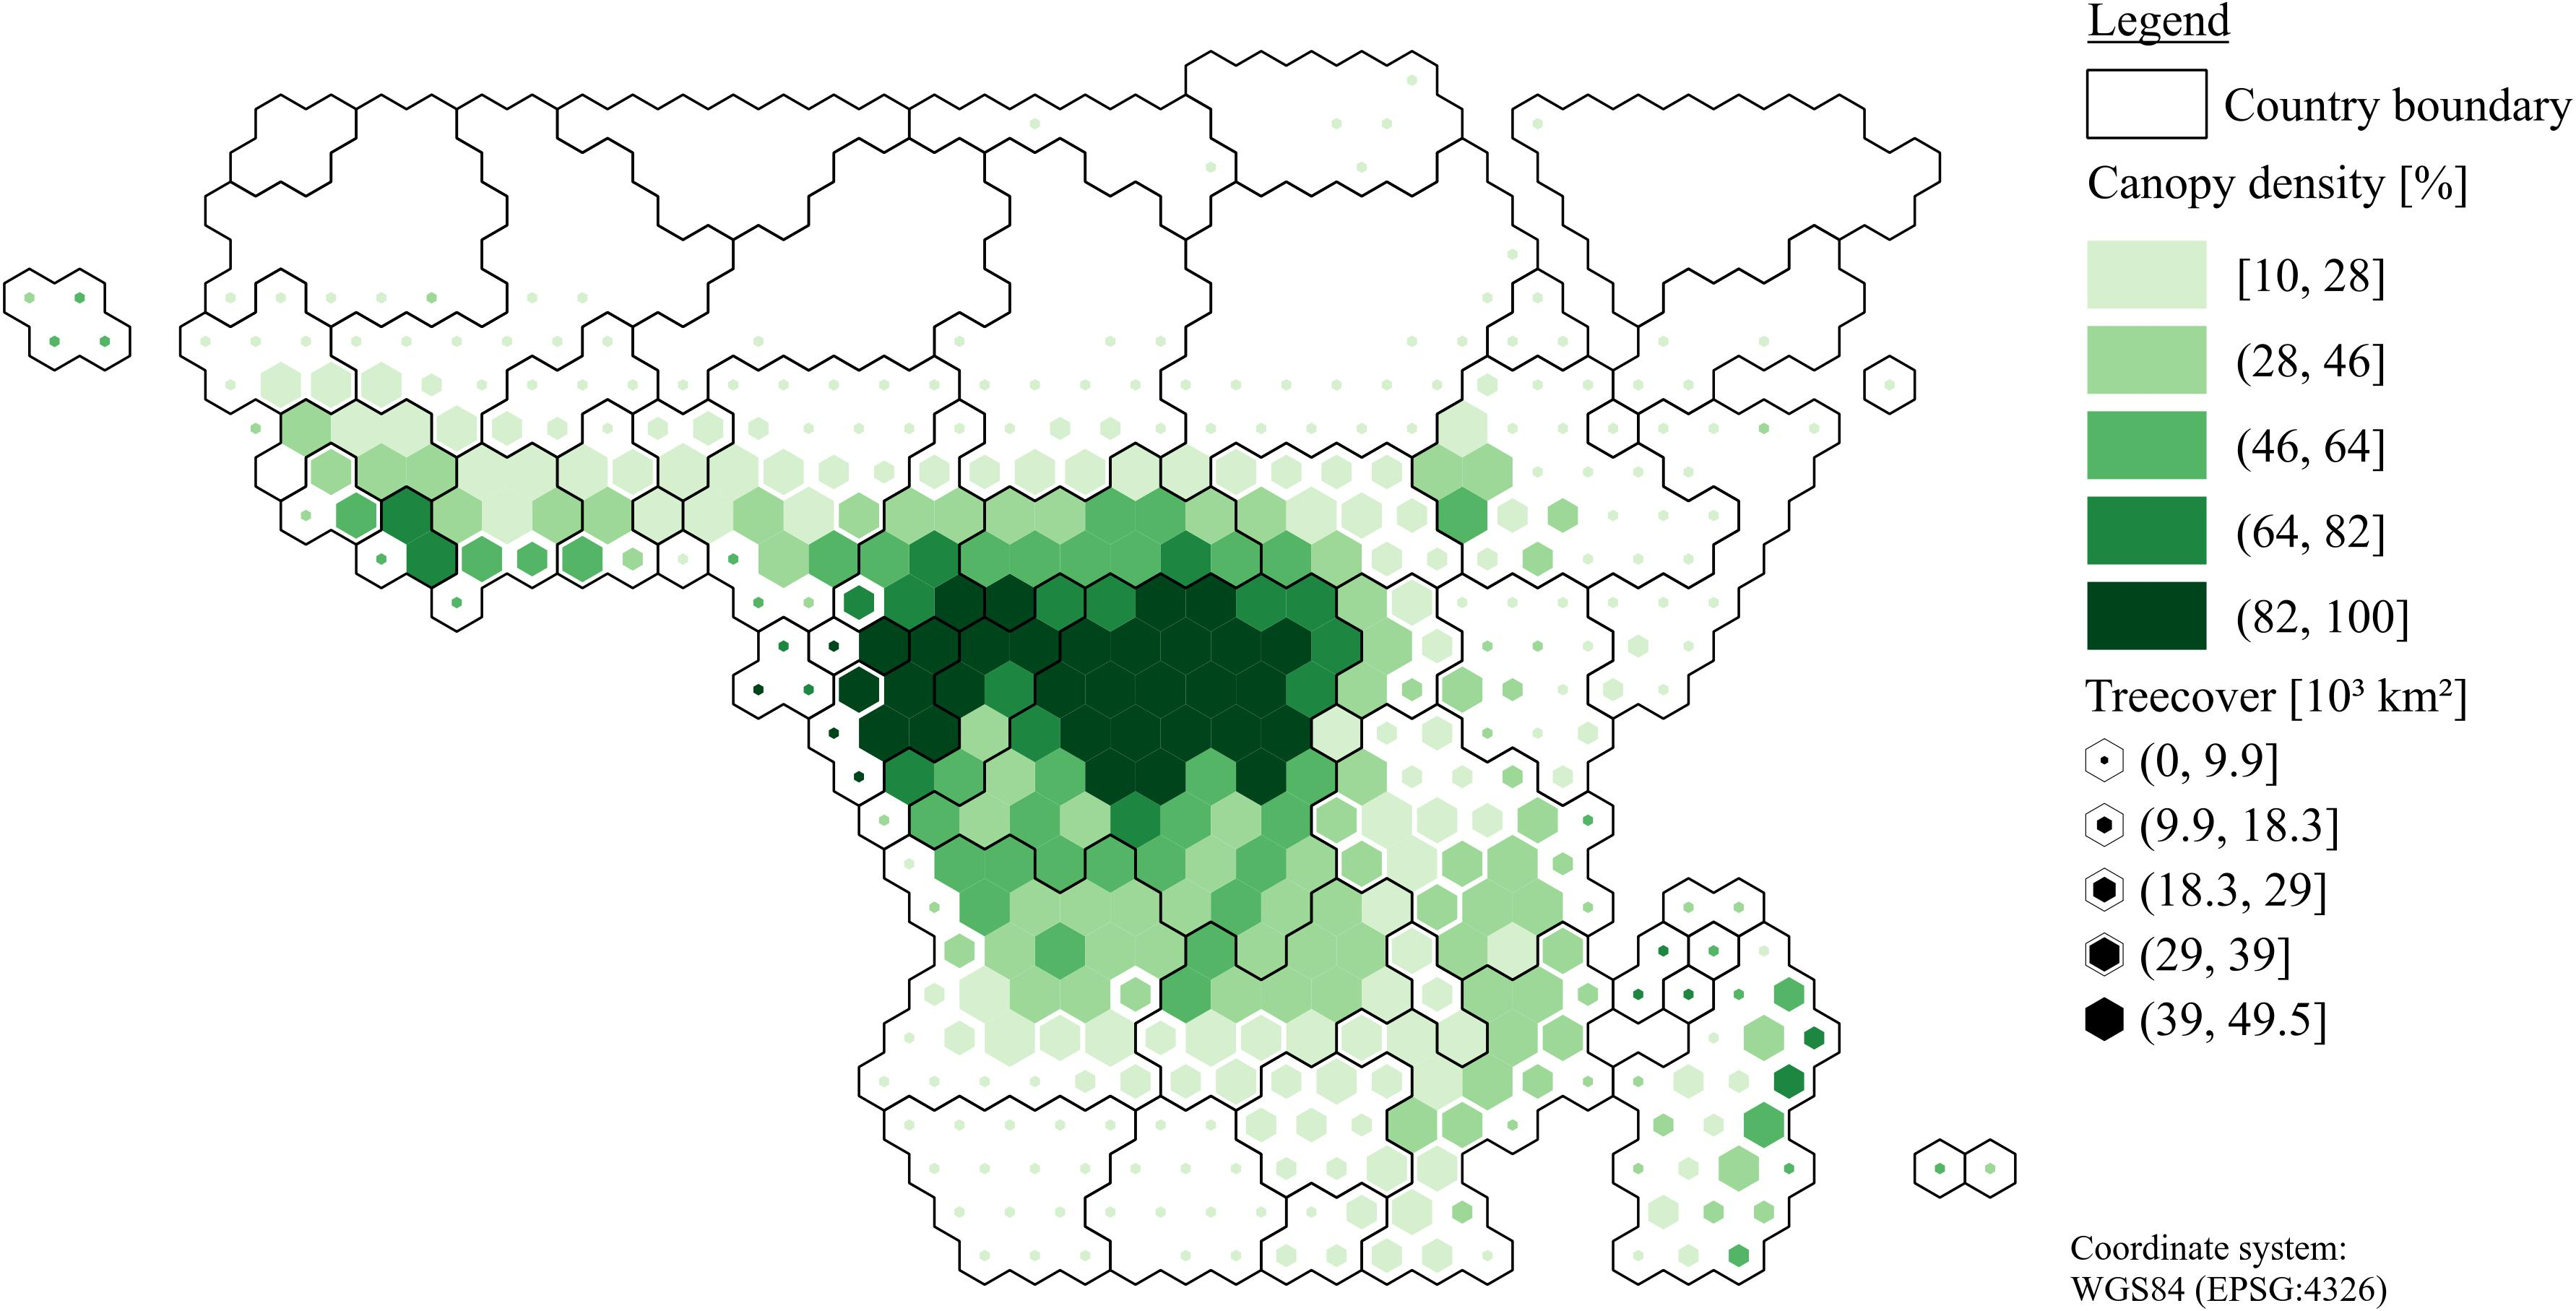
\includegraphics[scale=1]{img/africa_treecover_frameless}
%				\caption[Ecosystem service values]{}
%				\label{fig:africacover}
%			\end{figure}
%			\begin{figure}[ht]
%				\centering
%				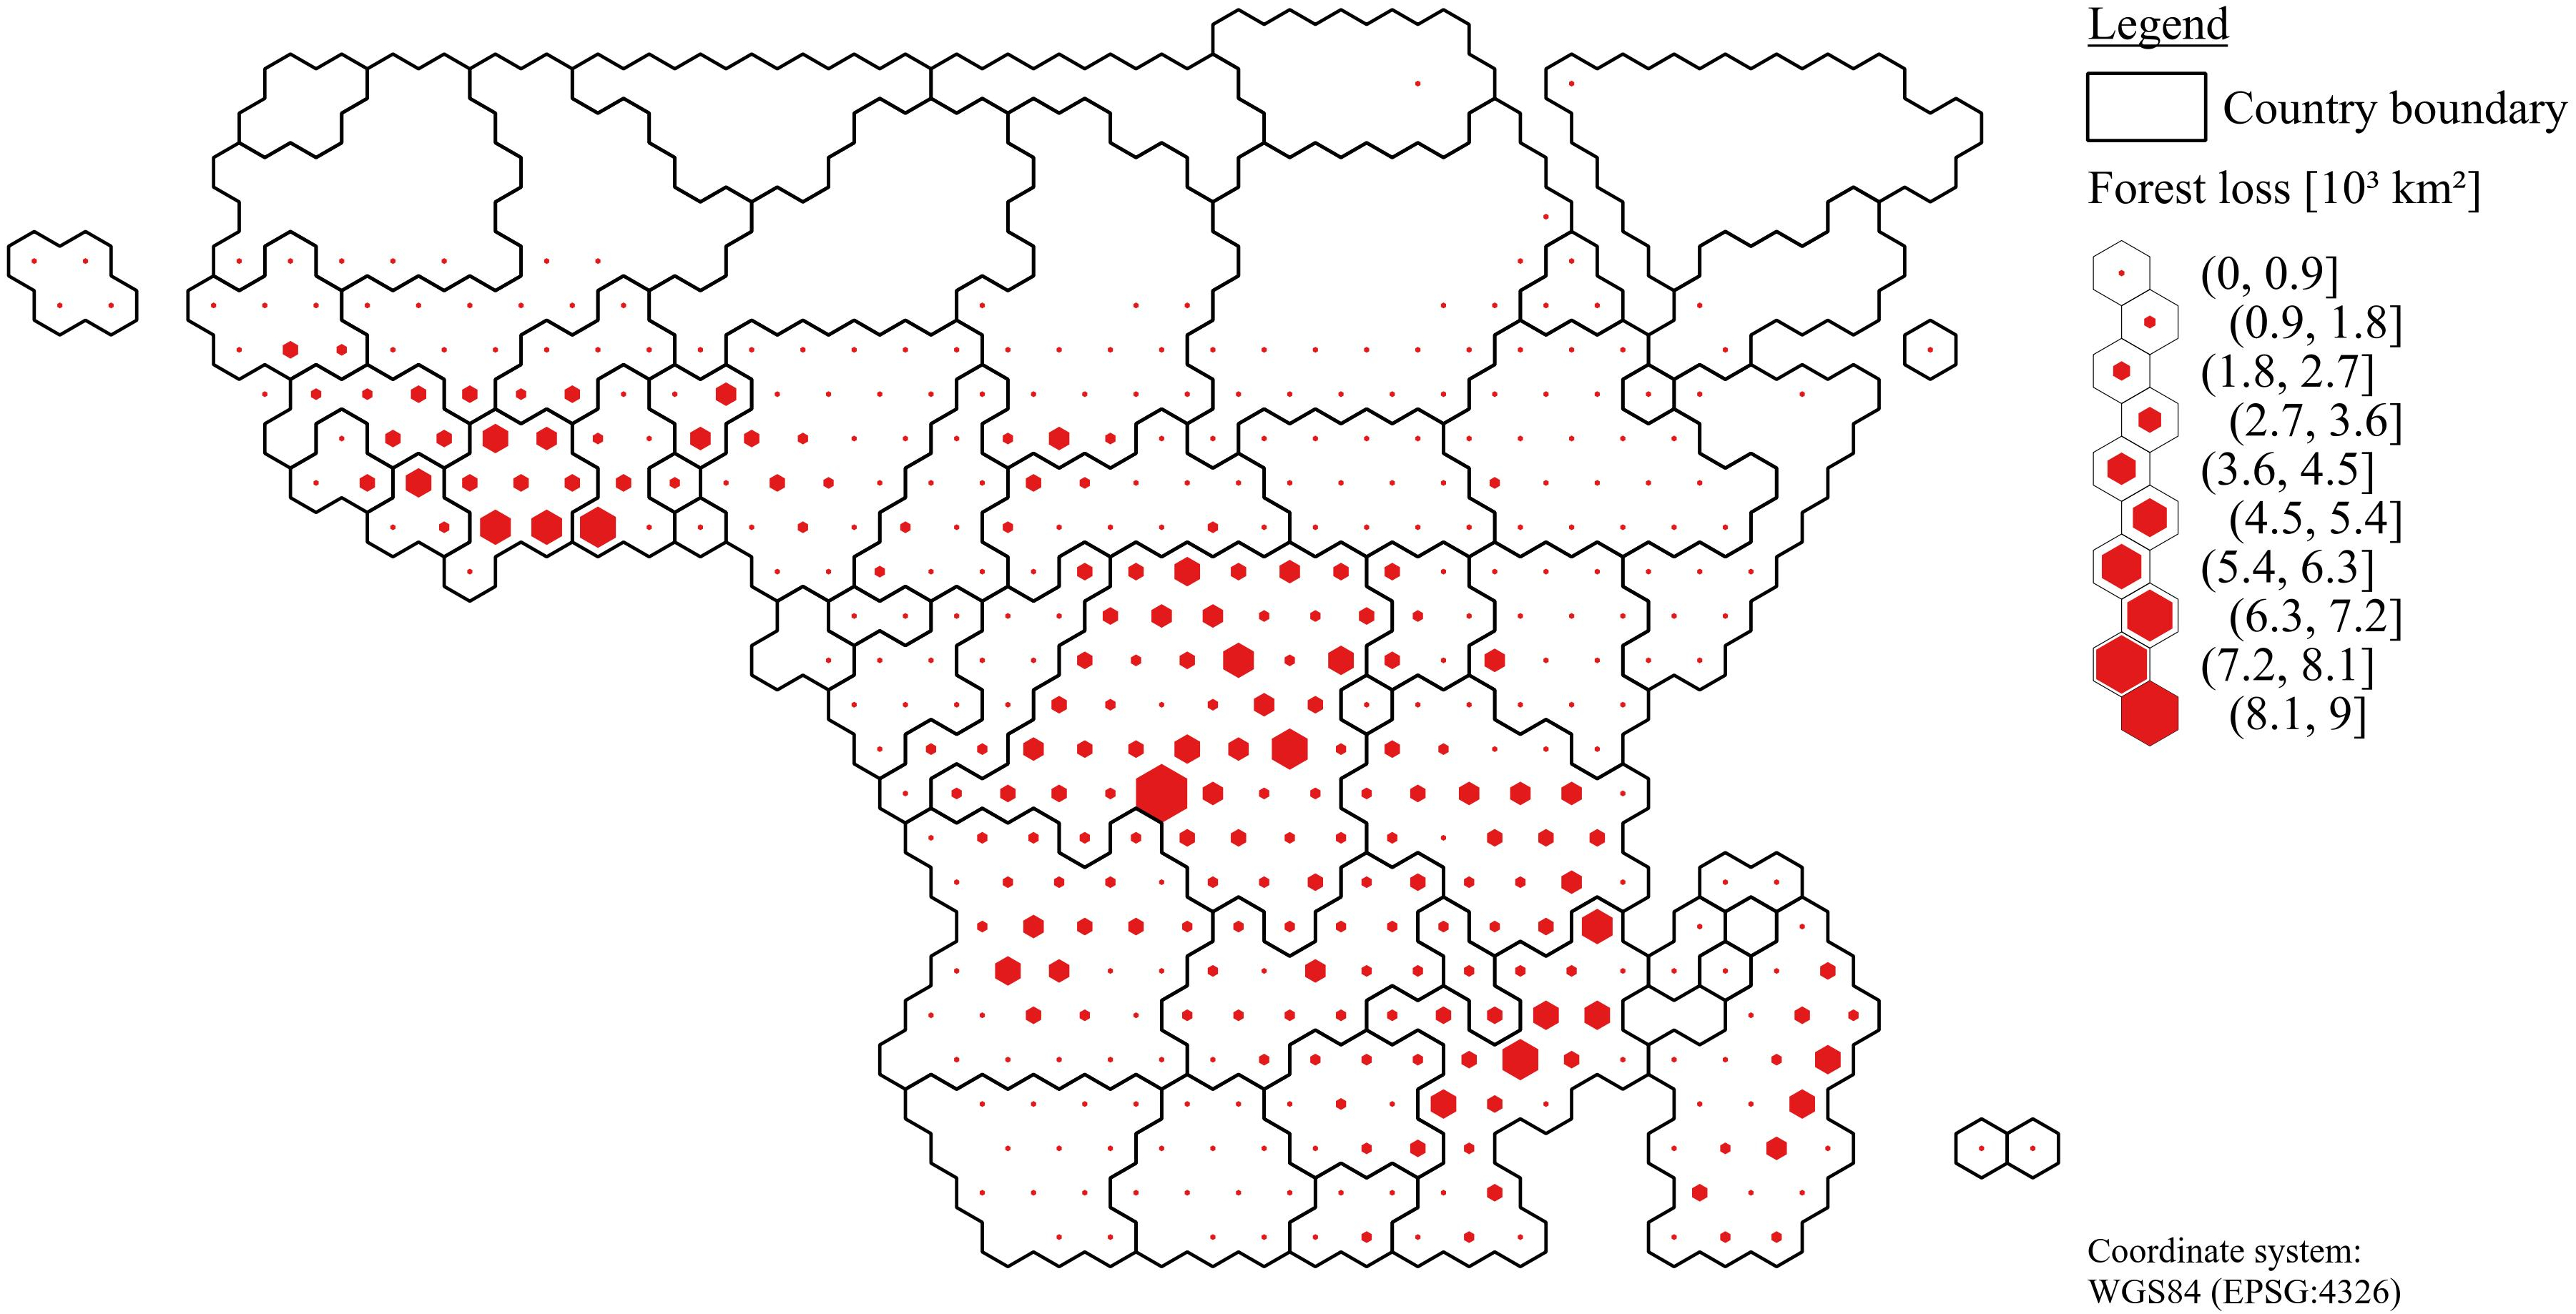
\includegraphics[scale=1]{img/africa_loss_frameless}
%				\caption[Ecosystem service values]{}
%				\label{fig:africaloss}
%			\end{figure}
%			\begin{figure}[ht]
%				\centering
%				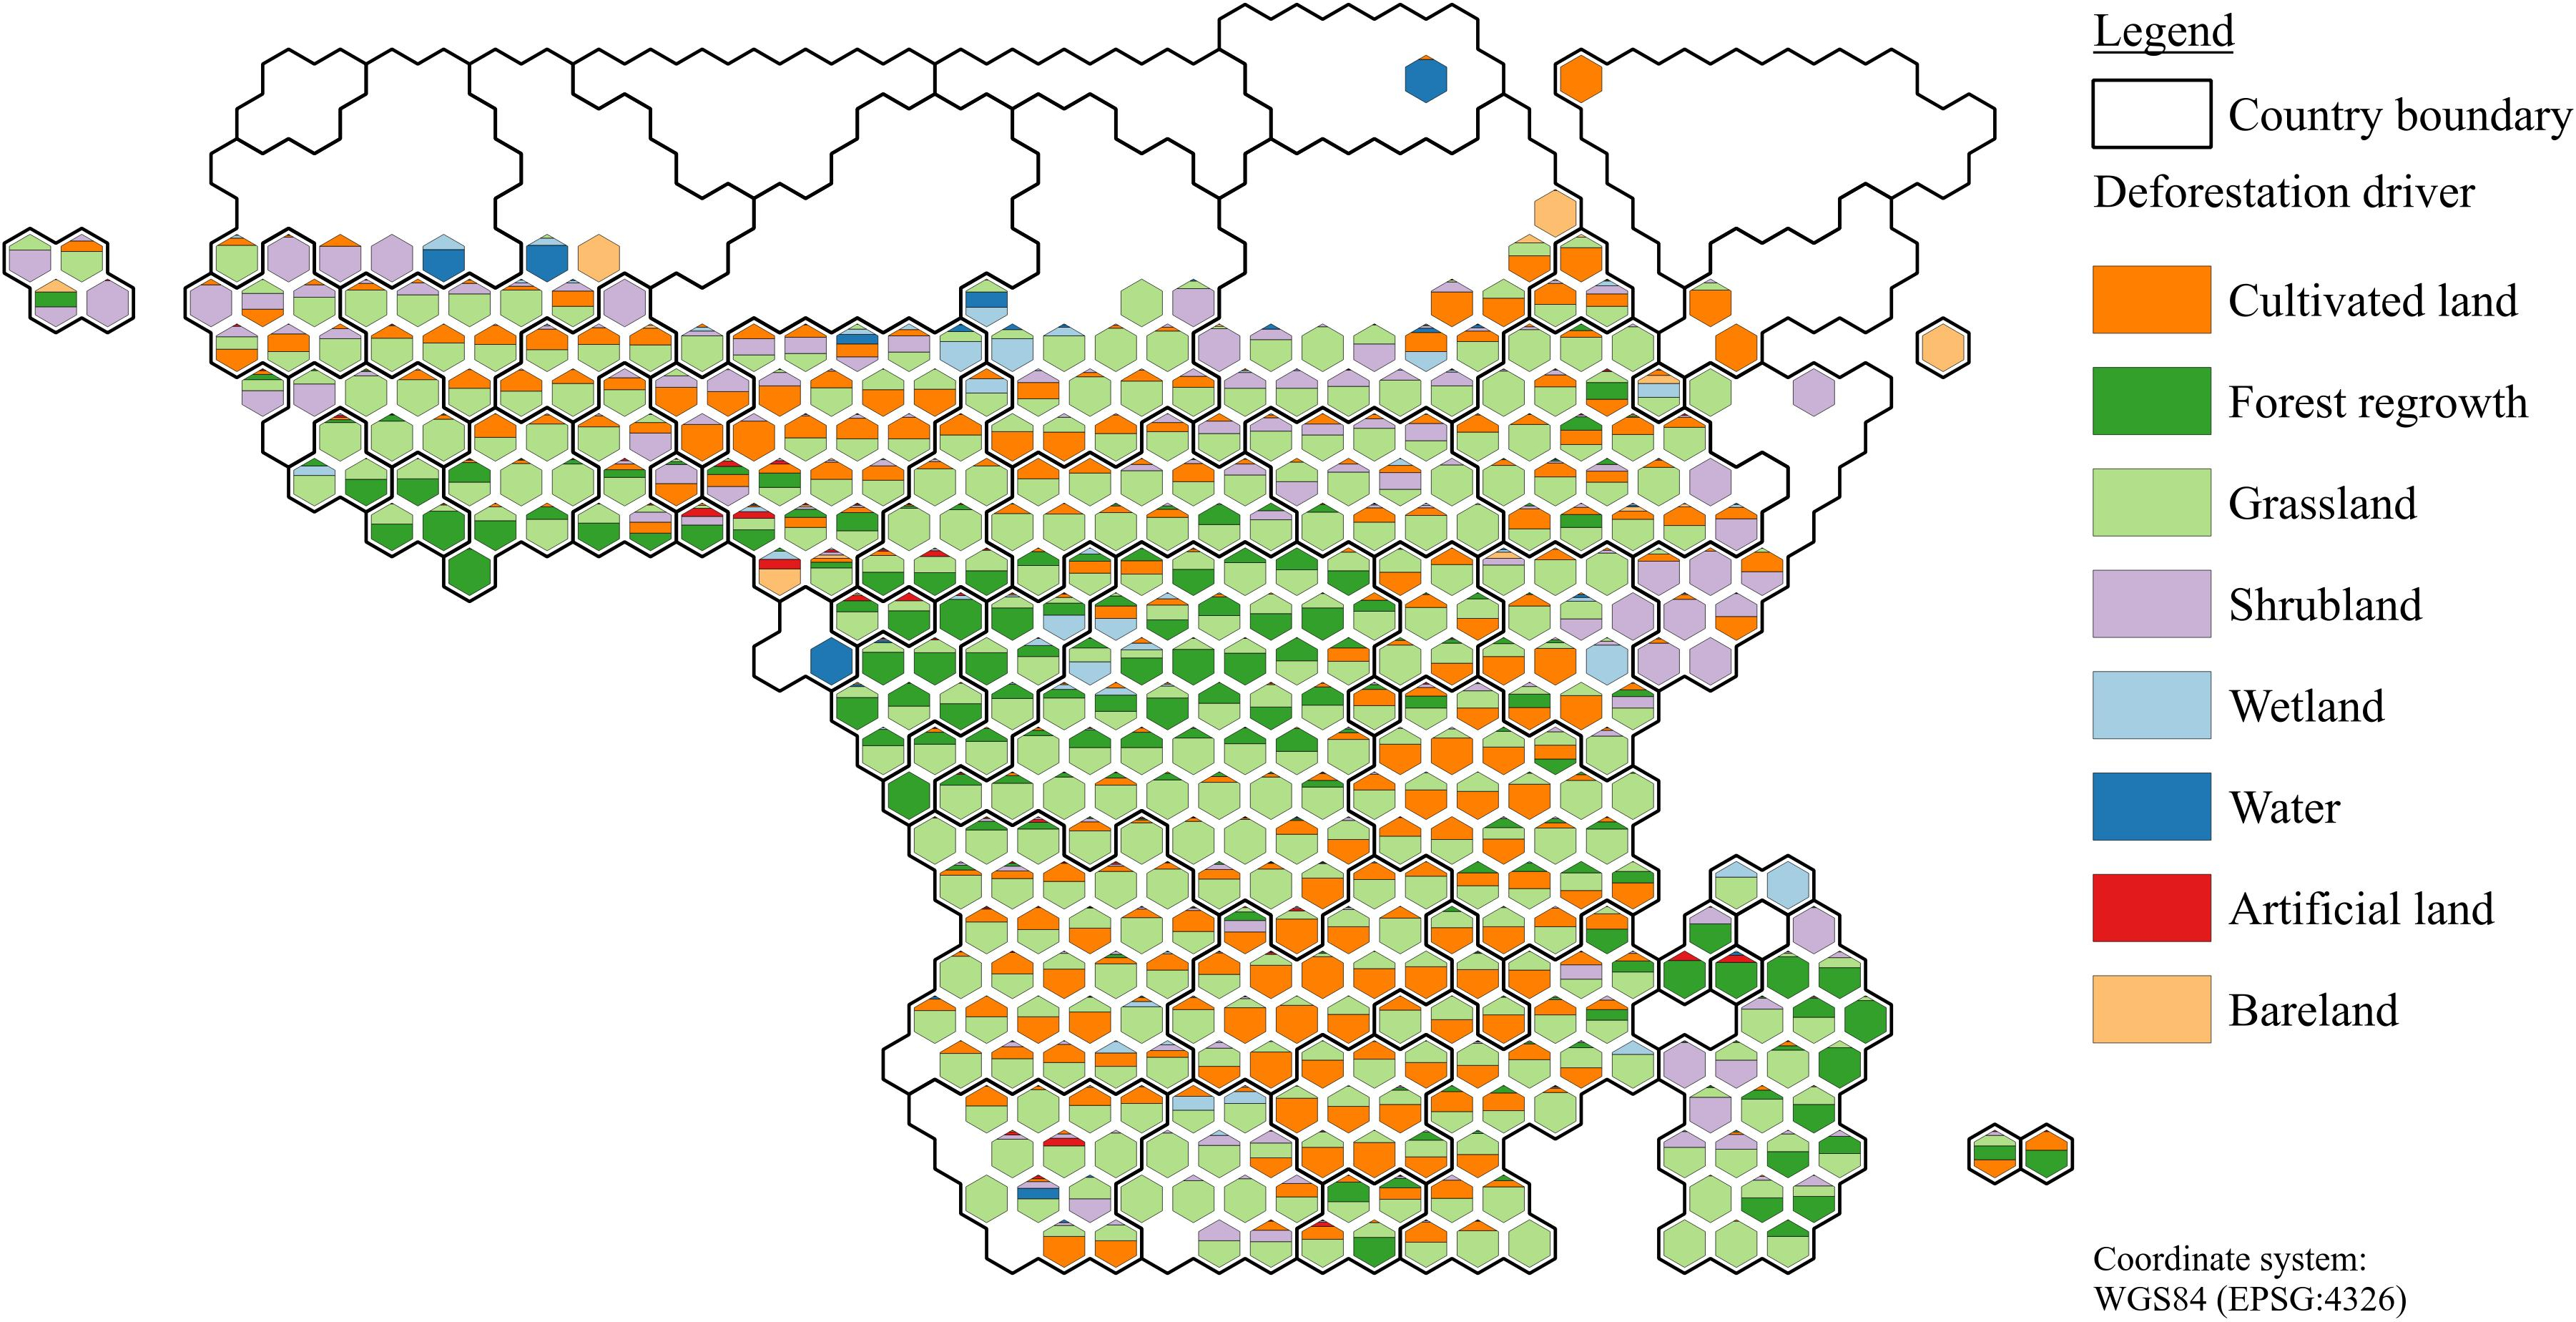
\includegraphics[scale=1]{img/africa_driver_frameless}
%				\caption[Ecosystem service values]{}
%				\label{fig:africadriver}
%			\end{figure}


% EMISSIONS
%		\begin{figure}[ht]
%			\centering
%			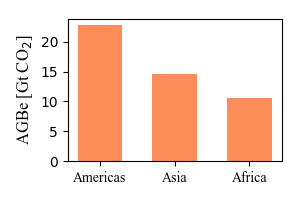
\includegraphics[scale=1]{img/agbe}
%			\caption[Ecosystem service values]{}
%			\label{fig:agbe}
%		\end{figure}
%		\begin{figure}[ht]
%			\centering
%			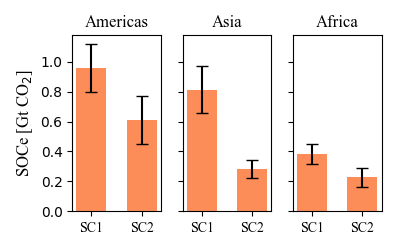
\includegraphics[scale=1]{img/soce}
%			\caption[Ecosystem service values]{}
%			\label{fig:soce}
%		\end{figure}
%
%		\begin{table}[ht]
%			\centering
%			\caption[Soil organic carbon emissions]{Soil organic carbon emissions}
%			\label{tab:soce_tab}
%			\begin{tabular}{lrrrrrrrrr}
%				\hline
%				\multirow{3}{*}{Region} & \multicolumn{3}{c}{SC1}& \multicolumn{3}{c}{SC2} & \multicolumn{3}{c}{SC3} \\
%				& \multicolumn{3}{c}{[Gt CO$_2$]}& \multicolumn{3}{c}{[Gt CO$_2$]} & \multicolumn{3}{c}{[Gt CO$_2$]} \\
%				& min & mean & max & min & mean & max & min & mean & max \\\hline
%				Americas & 0.80 & 0.96 & 1.12 & 0.45 & 0.61 & 0.77 & 0.43 & 0.59 & 0.76 \\
%				Asia & 0.66 & 0.81 & 0.97 & 0.22 & 0.28 & 0.34 & 0.22 & 0.28 & 0.33 \\
%				Africa & 0.32 & 0.39 & 0.45 & 0.17 & 0.23 & 0.29 & 0.16 & 0.23 & 0.29 \\\hline
%			\end{tabular}
%		\end{table}


% ESV
%		\begin{figure}[ht]
%			\centering
%			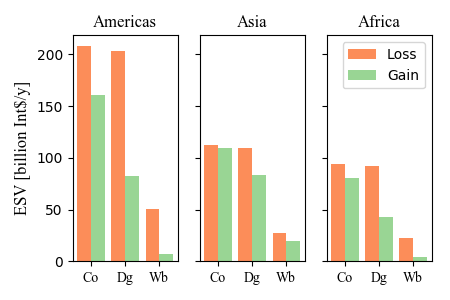
\includegraphics[scale=1]{img/esv}
%			\caption[Ecosystem service values]{}
%			\label{fig:esv}
%		\end{figure}


